% !TeX encoding = UTF-8
%% \textbf{重庆大学}通用毕业论文\LaTeXe{}模板
%%% 使用前请先阅读使用文档和用户协议,内有详细介绍。Happy Texing! :)
%% =======================================================
\documentclass%
	[type=master, bilinguallist=apart, 
	printmode=oneside, blindtrail=true]{cquthesis}%
% 可用选项:
% type=[bachelor|master|doctor],      % 必选,毕业论文类型,以下项目不填时为默认
% liberalformat,                      % 可选,仅适用本科生,使用文学类论文标题格式,默认未打开
% proffesionalmaster=[true|false],    % 可选,仅适用研究生,是(true)否(false)专业硕士,默认为否
% printmode=[oneside|twoside|auto],	  % 可选,论文打印方式,默认采用auto按页数要求自动判定
% openany,|openright,                 % 可选,双面打印时每章的第一页仅右页开启,默认右页开启(openright)
% bilinguallist=[off|combined|apart], % 可选,图录表录等分别按双语题注混编(combined),分开编录(apart),默认关(off)
% blindtrail=[true|false],                         % 可选,盲审模式,开启后封面姓名和致谢部分会隐藏,详情请参阅用户文档,默认关
% draft,                              % 写作期间可选,不渲染图片,关闭外围功能,加快预览速度,默认未开启

% 请在cquthesis.sty文件中定义其他会用到的宏包和自己的变量
% 这样可以防止main.tex太过臃肿。
\usepackage{cquthesis}

% 定义所有的图片文件在 figures 子目录下
\graphicspath{{figures/}}

% 定义数字圆
\usepackage{tikz}
\newcommand*\circled[1]{\tikz[baseline=(char.base)]{
            \node[shape=circle,draw,inner sep=1pt] (char) {\small #1};}}

%*** 写作时,使用这个命令只渲染你想查看的部分,提升工作效率,定稿时注释掉整行
% \includeonly{contents/introduction}
% \includeonly{contents/related_work}
% \includeonly{contents/MGRCL}
% \includeonly{contents/S2V}


\begin{document}


\cqusetup{
%	************	注意	************
%	* 1. \cqusetup{}中不能出现全空的行,如果需要全空行请在行首注释
%	* 2. 不需要的配置信息可以放心地坐视不理、留空、删除或注释(都不会有影响)
%	*
%	********************************
% ===================
%	论文的中英文题目
% ===================
  ctitle = {待补充},
  etitle = {待补充},
% ===================
% 作者部分的信息
% \secretize{}为盲审标记点,在打开盲审开关时内容会自动被替换为***输出,盲审开关默认关闭
% ===================
  cauthor = \secretize{尹国伟},	% 你的姓名,以下每项都以英文逗号结束
  eauthor = \secretize{Guowei~Yin},	% 姓名拼音,~代表不会断行的空格
  studentid = \secretize{},	% 仅本科生,学号
  csupervisor = \secretize{黄~~~晟~~~~~教授},	% 导师的姓名
  esupervisor = \secretize{{Prof.~Sheng Huang}},	% 导师的姓名拼音
  cassistsupervisor = \secretize{}, % 本科生可选,助理指导教师姓名,不用时请留空为{}
  cextrasupervisor = \secretize{}, % 本科生可选,校外指导教师姓名,不用时请留空为{}
  eassistsupervisor = \secretize{}, % 本科生可选,助理指导教师或/和校外指导教师姓名拼音,不用时请留空为{}
  cpsupervisor = \secretize{}, % 仅专硕,兼职导师姓名
  epsupervisor = \secretize{},	% 仅专硕,兼职导师姓名拼音
  cclass = \secretize{\rmfamily{2025}\heiti{年}\rmfamily{5}\heiti{月}},	% 博士生和学硕填学科门类,学硕填学科类型
  research_direction = \zihao{3}{工学},
  edgree = {},	% 专硕填Professional Degree,其他按实情填写
% % 提示:如果内容太长,可以用\zihao{}命令控制字号,作用范围:{}内
  cmajor = 工~~~~学,	% 专硕不需填,填写专业名称
  emajor = , % % 专硕不需填,填写专业英文名称
  cmajora = \zihao{3}{软件工程},
  cmajorb = \zihao{3}{计算机视觉},
  cmajorc = \secretize{},
  % cmajord = 2024年6月,
% ===================
% 底部的学院名称和日期
% ===================
  cdepartment = ,	%学院名称
  edepartment = ,	%学院英文名称
% ===================
% 封面的日期可以自动生成(注释掉时),也可以解除注释手动指定,例如:二〇一六年五月
% ===================
%	mycdate = {2023年6月},
%	myedate = {June 2023},
}% End of \cqusetup
% ===================
%
% 论文的摘要
%
% ===================
\begin{cabstract}	% 中文摘要
针对问题一,首先将题目中 BT.2020 和显示屏色域(sRGB)的色度坐标转换为"设备无关"的 XYZ 三刺激值,并基于此三刺激值转换为 CIELab 空间。我们选择专业的广泛使用的 $\Delta E_{2000}$ 色差公式,并以其为优化目标,使用差分进化算法对其进行优化。最后得到视频源色域到显示屏色域的 XYZ 三刺激值转换矩阵。将转换后的结果与原显示屏色域相比可以得到极低的 $\Delta E_{2000}$ 损失值以及色度图面积差值。说明此模型具有极低的感知误差以及对目标色域的高保真拟合。

针对问题二,我们通过训练一个神经网络来学习从四通道RGBV输入到五通道RGBCX输出的映射关系。为此,设计了一个 ColorNet(一个简单的多层感知器),其输入层接收4个特征(RGBV),输出层产生5个特征(RGBCX)。训练过程使用了一个合成数据集,该数据集通过受控的非线性变换生成,以模拟现实世界的复杂性。最小化颜色转换损失的关键在于自定义的 CombinedLoss 函数。该函数结合了两种损失成分:均方误差(MSE),$\Delta E_{2000}$,通过对这两种损失成分进行加权,模型在保持整体通道一致性的同时,优先考虑感知上准确的色彩再现。模型使用AdamW优化器进行训练,并通过跟踪训练损失和验证损失来评估其性能。最后,解决方案包括ΔE2000误差分布、输入和输出系统色域的色度图以及样本颜色预测的可视化,以评估学习到的映射的有效性。

针对问题三,建立了基于CIE Lab色彩空间和三基色原理的LED显示器颜色校正模型。该模型结合伽马校正与线性矩阵变换,采用差分进化算法优化校正参数,实现精确的颜色还原。首先,通过对数线性回归估计LED显示器的伽马参数,发现主色通道(如红色图像的R通道)的伽马值显著较小(约0.022),而非主色通道的伽马值相对较大(约0.23),体现了LED显示器在不同颜色通道上的非线性响应特性差异。然后,设计包含色差损失、正则化项和行列式惩罚的综合目标函数,基于CIE $\Delta E_{00}$色差公式构建优化目标。采用全局-局部混合优化策略:先用差分进化算法进行全局搜索,再用L-BFGS-B方法进行局部精调。实验结果表明,三种基色图像的平均色差从2.0以上降低到0.1左右,平均改善幅度达95.6\%;校正后100\%像素的色差均小于1.0,达到人眼难以察觉的优秀标准;校正矩阵行列式值约0.10,保证了数值稳定性和变换可逆性。该模型为LED显示器颜色处理提供了完整的理论框架和实用的工程解决方案。
\end{cabstract}
% 中文关键词,请使用英文逗号分隔:
\ckeywords{颜色空间转换;LED显示器校正;CIE Lab色彩空间;$\Delta E_{00}$色差;差分进化;神经网络;伽马校正;多通道颜色系统}

% 封面和摘要配置完成
% 封面部分
% \makecover

\frontmatter %%%前置部分(封面后绪论前)
\cquauthpage[contents/cover1.pdf]
%\cquauthpage[contents/cover2.pdf]
%\cquauthpage[contents/cover3.pdf]
%\cquauthpage[contents/cover4.pdf]

%% 原创声明和授权说明书,可选:用扫描页替换
%\cquauthpage[authscan.pdf]
%\cquauthpage

% 摘要
\makeabstract

%% 目录,注意需要多次编译才能更新
\setlength{\cftbeforetoctitleskip}{0pt}
\setlength{\cftaftertoctitleskip}{20pt}
\tableofcontents


% \setlength{\cftbeforelottitleskip}{0pt}
% \setlength{\cftafterlottitleskip}{20pt}
%% 插图索引,可选,如不用可注释掉
\renewcommand*{\listfigurename}{图目录}
\clearpage
\phantomsection
\addcontentsline{toc}{chapter}{图目录}
\listoffigures
%\listoffiguresEN
% \setlength{\cftbeforelottitleskip}{0pt}
% \setlength{\cftafterlottitleskip}{20pt}
%% 表格索引,可选
\renewcommand*{\listtablename}{表目录}
\clearpage
\phantomsection
\addcontentsline{toc}{chapter}{表目录}
\listoftables
%\listoftablesEN
%% 公式索引,可选
%\listofequations
%\listofequationsEN
%% 符号对照表,可选
% \clearpage
% \phantomsection 
% \addcontentsline{toc}{chapter}{主要符号对照表}
% % !TeX encoding = UTF-8
% 环境用两个长度参数,分别定义左边距以及词条和解释的水平距离,可自己调试以达美观(全去掉时默认:20mm,30mm)
\begin{denotation}[0mm][15mm]
	% 颜色空间相关符号
	\item[$M$] 颜色空间转换矩阵 $M\in \mathbb{R}^{3\times 3}$
	\item[$\mathbf{c}_i$] 第$i$个BT.2020 RGB颜色样本 $\mathbf{c}_i \in [0,1]^3$
	\item[$\mathbf{c}'_i$] 映射后的显示屏RGB颜色样本
	\item[$M_{BT\rightarrow XYZ}$] BT.2020色域到XYZ色彩空间的转换矩阵
	\item[$M_{DP\rightarrow XYZ}$] 显示屏色域到XYZ色彩空间的转换矩阵
	\item[$L^*$] CIE Lab色彩空间中的明度分量
	\item[$a^*$] CIE Lab色彩空间中的红绿轴分量
	\item[$b^*$] CIE Lab色彩空间中的黄蓝轴分量
	\item[$\Delta E_{00}$] CIE DE2000色差公式
	\item[$X, Y, Z$] CIE XYZ色彩空间的三刺激值
	\item[$x, y$] CIE 1931色度图坐标
	\item[$\overline{x}(\lambda), \overline{y}(\lambda), \overline{z}(\lambda)$] CIE 1931标准色度观察者匹配函数
	\item[$S(\lambda)$] 光谱功率分布函数
	
	% 神经网络相关符号
	\item[$\mathbf{X}$] 神经网络输入数据矩阵,4通道RGBV
	\item[$\mathbf{Y}$] 神经网络目标输出数据矩阵,5通道RGBCX
	\item[$W$] 神经网络权重矩阵
	\item[$\mathbf{b}$] 神经网络偏置向量
	\item[$f(\cdot)$] 激活函数
	\item[$L_{MSE}$] 均方误差损失函数
	\item[$L_{\Delta E_{2000}}$] 基于$\Delta E_{2000}$的感知误差损失函数
	\item[$L_{total}$] 混合损失函数
	\item[$\alpha, \beta$] 损失函数权重参数
	\item[$\eta$] 学习率
	
	% 差分进化算法相关符号
	\item[$\mathbf{x}_i$] 差分进化算法中第$i$个个体
	\item[$NP$] 差分进化算法种群大小
	\item[$F$] 差分进化算法变异因子
	\item[$CR$] 差分进化算法交叉概率
	\item[$\mathbf{v}_i$] 差分进化算法变异向量
	\item[$\mathbf{u}_i$] 差分进化算法试验向量
	\item[$G$] 差分进化算法迭代代数
	
	% LED颜色校正相关符号
	\item[$\gamma_c$] 第$c$个颜色通道的伽马值
	\item[$S_c$] 第$c$个颜色通道的比例因子
	\item[$I_{\text{meas},c}$] 第$c$个颜色通道的测量值
	\item[$I_{\text{target},c}$] 第$c$个颜色通道的目标值
	\item[$\mathbf{x}$] 线性RGB向量 $\mathbf{x} = [R_\ell, G_\ell, B_\ell]^T$
	\item[$\mathbf{y}$] 校正后RGB向量
	\item[$L_{\mathrm{DE}}$] 基于CIE $\Delta E_{00}$的色差损失
	\item[$L_{\mathrm{reg}}$] 正则化损失项
	\item[$L_{\det}$] 行列式惩罚项
	\item[$\mathcal{L}(M,\mathbf{b})$] LED颜色校正总目标函数
	\item[$\lambda_1, \lambda_2, \lambda_3$] 损失函数权重参数
	\item[$\epsilon$] 行列式惩罚阈值
	\item[$\text{clip}$($\cdot$, [0,1])] 数值裁剪函数,限制在[0,1]范围
	
	% 数学运算符号
	\item[$\|\cdot\|_F$] Frobenius范数
	\item[$\|\cdot\|_2$] 欧几里得范数
	\item[$\det(\cdot)$] 矩阵行列式
	\item[$I_3$] $3 \times 3$单位矩阵
	\item[$\mathbf{1}(\cdot)$] 指示函数
	\item[$\lor$] 逻辑或运算符
	
	% 其他常用符号
	\item[$N$] 样本数量
	\item[$k$] 样本索引
	\item[$c$] 颜色通道索引,$c \in \{R,G,B\}$
	\item[$\text{popsize}$] 差分进化算法种群大小
	\item[$\text{maxiter}$] 最大迭代次数
	\item[$D65$] 标准光源D65白点
	\item[$\delta$] CIE Lab转换中的阈值参数,$\delta = 6/29$
\end{denotation}

\endinput
% %% 缩略语对照表,可选
% \clearpage
% \phantomsection 
% \addcontentsline{toc}{chapter}{缩略语对照表}
% \input{contents/abbreviate}

\mainmatter %%% 主体部分(绪论开始,结论为止)
%* 子文件的多少和内容由你决定(最好以章为单位),基本原则是提速预览、脉络清晰、管理容易。

% 设置字号为小四
\renewcommand{\normalsize}{\fontsize{12pt}{20pt}\selectfont}
% 设置小四正文行间距为 20 磅
\setstretch{1.312}

\chapter[\hspace{0pt}绪论]{{\heiti\zihao{3}\hspace{0pt}绪\hskip\ccwd{}论}}\label{chapter: 绪论}
dawd\cite{MAML}
\section[\hspace{-2pt}研究背景与意义]{{\heiti\zihao{-3} \hspace{-8pt}研究背景与意义}}\label{section1: 研究背景与意义}

\section[\hspace{-2pt}问题提出与研究内容]{{\heiti\zihao{-3} \hspace{-8pt}问题提出与研究内容}}\label{section1: 问题提出与研究内容}



\chapter[\hspace{0pt}问题分析]{{\heiti\zihao{3}\hspace{0pt}问题分析}}

\removelofgap
\removelotgap

\section[\hspace{-2pt}问题重述]{{\heiti\zihao{-3} \hspace{-8pt}问题重述}}\label{section2: 问题重述}

\section[\hspace{-2pt}模型假设]{{\heiti\zihao{-3} \hspace{-8pt}模型假设}}\label{section2: 模型假设}


\section[\hspace{-2pt}符号定义]{{\heiti\zihao{-3} \hspace{-8pt}符号定义}}\label{section2: 符号定义}



\section[\hspace{-2pt}理论基础]{{\heiti\zihao{-3} \hspace{-8pt}理论基础}}\label{section2: 理论基础}


为了便于对后续视频源BT.2020色域与普通显示屏RGB色域之间映射关系的分析,我们首先引入标准色度系统的数学模型,对常见色彩空间进行建模表示。这些空间构成了本问题中色彩转换和损失评估的基础框架。

\subsection[\hspace{-2pt}CIE1931标准色度观察者与光谱三刺激值]{{\heiti\zihao{4} \hspace{-8pt}CIE1931标准色度观察者与光谱三刺激值}}\label{section2: CIE1931标准色度观察者与光谱三刺激值}
CIE 1931是是由国际照明委员会(CIE)于1931年定义的色彩模型,其核心在于基于实验测量建立的“标准色度观察者”响应曲线。这一模型通过三条匹配函数 $\overline{x}(\lambda),\overline{y}(\lambda),\overline{z}(\lambda) $ 将任意波长下的光谱功率分布(SPD)映射为三刺激值(Tristimulus Values):
\begin{equation}
\begin{aligned}
  &X = \int_{\lambda}S(\lambda)\overline{x}(\lambda)d\lambda,\ \ \ Y = \int_{\lambda}S(\lambda)\overline{y}(\lambda)d\lambda,\ \ \ Z = \int_{\lambda}S(\lambda)\overline{z}(\lambda)d\lambda
\end{aligned}
\end{equation}

\subsection[\hspace{-2pt}CIEXYZ颜色空间]{{\heiti\zihao{4} \hspace{-8pt}CIEXYZ颜色空间}}\label{section2: CIEXYZ颜色空间}
CIEXYZ 是一个以三刺激值为基础的线性色彩空间,被视为“设备无关”的色彩表示方式。其三个分量 $(X,Y,Z)$ 分别对应红、绿、蓝三种感知通道。Y 分量也通常用作\textbf{亮度(Luminance)}的代表。该空间是许多其他色彩空间(如 Lab、sRGB、BT.2020)的中间标准基础。通常不同色域之间的转换以此为中介。

\subsection[\hspace{-2pt}CIELab颜色空间]{{\heiti\zihao{4} \hspace{-8pt}CIELab颜色空间}}\label{section2: CIELab颜色空间}
CIELab 空间是基于 CIEXYZ 空间定义的感知均匀色彩空间,能够更好地符合人眼对颜色差异的敏感性。其由以下三个分量构成:
\begin{equation}
\begin{aligned}
  &L^{*}\ ,\ \ a^{*}\ ,\ \ b^P{*}\ 
\end{aligned}
\end{equation}
其中,$L^{*}$代表明度,$a^{*}$代表红绿轴,$b^{*}$代表黄蓝轴。具体变换公式如下(以D65白点为例):
\begin{equation}
\begin{aligned}
  &f(t) = 
\begin{cases}
  t^{\frac{1}{3}}\ \ \ \ t>\delta^{3}\\
  \frac{t}{3\delta^{2}}+\frac{4}{29}\ \ \ \ t\leq \delta^{3}\\
\end{cases}
,\ \ \delta=\frac{6}{29}
\end{aligned}
\end{equation}

\begin{equation}
\begin{aligned}
  &L^{*} = 116f(\frac{Y}{Y_{n}})-16,\ \ \ a^{*}=500[f(\frac{X}{X_{n}})-f(\frac{Y}{Y_{n}})],\ \ \ b^{*} = 200[f(\frac{Y}{Y_{n}})-f(\frac{Z}{Z_{n}})]
\end{aligned}
\end{equation}

其中$(X_{n},Y_{n},Z_{n})$ 为参考白点(如D65)的三刺激值。

\subsection[\hspace{-2pt}CIE1931xy色度图与色域表示]{{\heiti\zihao{4} \hspace{-8pt}CIE1931xy色度图与色域表示}}\label{section2: CIE1931xy色度图与色域表示}
CIEXYZ 空间中颜色可以通过如下变换得到色度图中的坐标:

\begin{equation}
\begin{aligned}
  &x=\frac{X}{X+Y+Z},\ \ y=\frac{Y}{X+Y+Z}
\end{aligned}
\end{equation}

该色度图表示了所有可见光的二维投影范围,设备的色域可以通过其三基色的 $(x,y)$ 点连线形成三角形表示。色域越大,所能表示的颜色越丰富。该图是色彩匹配与色彩损失分析的重要工具。

\subsection[\hspace{-2pt}CIEDE2000色差公式]{{\heiti\zihao{4} \hspace{-8pt}CIEDE2000色差公式}}\label{section2: CIEDE2000色差公式}


为了更精确的对问题进行建模并且便于后续损失函数以及差分进化算法的实现,我们将题目中的BT.2020颜色空间以及显示屏的颜色空间从 xy 色度坐标转换为 XYZ 颜色空间,再利用 Lab 颜色空间公式转换为 $(L^{*},a^{*},b^{*})$ 。最后计算 $\Delta E_{00}$ 损失值。

在将 BT.2020 高清视频源的色彩空间映射至普通显示屏 RGB 色域时,由于显示设备色域较小,无法完整覆盖原始色域,导致部分颜色无法被准确再现。因此,我们需要设计一个合理的\textbf{色彩转换映射矩阵} $M\in \mathbb{R}^{3\times 3}$ ,以最小化从 BT.2020 色域到显示屏色域的映射过程中所产生的\textbf{主观感知误差}。

为度量这一色彩差异,应选择符合人眼视觉感知的度量方式。传统的欧几里得差异(如 RGB 或 XYZ 空间中的 L2 距离)不能很好地反映颜色感知误差。我们引入国际照明委员会(CIE)推荐的 $\Delta E_{00}$ 作为感知误差的度量函数。

对任意两个颜色在Lab空间中的向量:
\begin{equation}
\begin{aligned}
  &Lab_{1} = (L^{*}_{1},a^{*}_{1},b^{*}_{1}),\ \ \ Lab_{2}=(L^{*}_{2},a^{*}_{2},b^{*}_{2})
\end{aligned}
\end{equation}

$\Delta E_{00}$ 的计算公式如下:
\begin{equation}
\begin{aligned}
  &\Delta E_{00}=\sqrt{(\frac{\Delta L^{'}}{k_{L}S_{L}})^{2}+(\frac{\Delta C^{'}}{k_{C}S_{C}})^{2}+(\frac{\Delta H^{'}}{k_{H}S_{H}})^{2}+R_{T}\cdot{(\frac{\Delta C^{'}}{k_{C}S_{C}})}\cdot (\frac{\Delta H^{'}}{k_{H}S_{H}})}
\end{aligned}
\end{equation}
\textbf{(1)明度差与平均明度}
\begin{equation}
\begin{aligned}
   &\Delta L^{'} = L^{*}_{2}-L^{*}_{1},\ \ \overline{L}=\frac{L^{*}_{2}-L^{*}_{1}}{2}
\end{aligned}
\end{equation}
\textbf{(2)色度差与平均色度}
\begin{equation}
\begin{aligned}
  &C_{1}=\sqrt{a^{*2}_{1}+b^{*2}_{1}},\ \ C_{2}=\sqrt{a^{*2}_{2}+b^{*2}_{2}},\ \ \Delta C^{'}=C_{2}-C_{1},\ \ \overline{C}=\frac{C_{1}+C_2}{2}
\end{aligned}
\end{equation}
\textbf{(3)色相角差与平均色相角}
\begin{equation}
\begin{aligned}
 &h_{1}=\arctan2(b^{*}_{1},a^{*}_{1}),\ \ h_{2}=\arctan2(b^{*}_{2},a^{*}_{2})\\
 &\Delta h^{'}=h_{2}-h_{1},\ \ \Delta H^{1}=2\sqrt{C_{1}C_{2}}\sin (\frac{\Delta h^{'}}{2})\\
 &\overline{h}=
 \begin{cases}
   \frac{h_{1}+h_{2}}{2},\ \ |h_{1}-h_{2}|>180^{\circ}\\
   \frac{h_{1}+h_{2}+360^{\circ}}{2},\ \ |h_{1}-h_{2}|\leq 180^{\circ}
 \end{cases}
\end{aligned}
\end{equation}
\textbf{(4)调整因子}
\begin{equation}
\begin{aligned}
  &G=0.5(1-\sqrt{\frac{\overline{C^{7}}}{\overline{C^{7}}+25^{7}}})\\
  &T=1-0.17\cos(\overline{h}-30^{\circ})+0.24\cos(2\overline{h})+0.32\cos(3\overline{h}+6^{\circ})-0.20\cos(4\overline{h}-63^{\circ})
\end{aligned}
\end{equation}
\textbf{(5)权重因子}
\begin{equation}
\begin{aligned}
 &S_{L}=1+\frac{0.015(L-50)^{2}}{\sqrt{20+(\overline{L}-50)^{2}}},\ \ S_{C}=1+0.045\overline{C},\ \ S_{H}=1+0.015\overline{C}T
\end{aligned}
\end{equation}
\textbf{(6)旋转补偿因子}
\begin{equation}
\begin{aligned}
 &R_{T}=-\sin(2\Delta \theta)\cdot R_{C},\ \ \Delta \theta=30\exp\{-(\frac{\overline{h}-275^{\circ}}{25})^{2}\},\ \ R_{C}=2\sqrt{\frac{\overline{C^{7}}}{\overline{C^{7}}+25^{7}}}
\end{aligned}
\end{equation}
其中:$\Delta L^{'}$ :明度差,$\Delta C^{'}$ :色度差,$\Delta H^{'}$ :色相差,$S_{L},S_{C},S_{H}$ :感知缩放因子,$k_{L}=k_{C}=k_{H}=1$ :常用单位权重。

由上述公式,可以计算出两个 CIELab值 的色差。该函数对人眼感知差异具有良好拟合性能,因此被广泛用于图像质量、颜色匹配等领域。
\subsection[\hspace{-2pt}颜色感知与颜色空间]{{\heiti\zihao{4} \hspace{-8pt}颜色感知与颜色空间}}\label{section2: 颜色感知与颜色空间}

人类对颜色的感知是一个复杂的生理和心理过程。为了量化和描述颜色,引入了颜色空间的概念。常见的颜色空间包括:

\begin{itemize}
    \item \textbf{RGB (Red, Green, Blue)}:基于三原色加法混色的颜色模型,常用于显示设备和图像输入设备。然而,RGB 并非感知均匀,即欧氏距离不直接对应人眼感知的颜色差异。
    \item \textbf{XYZ (CIE 1931 XYZ)}:国际照明委员会 (CIE) 定义的一种基于人眼视觉生理特性的颜色空间。它涵盖了人眼可见的所有颜色,且与设备无关。其分量 $X, Y, Z$ 分别对应于光谱在人眼视锥细胞响应曲线下的积分。$Y$ 分量通常表示亮度信息。
    \item \textbf{Lab (CIE L*a*b*)}:一种感知均匀的颜色空间,从 XYZ 空间推导而来。$L^*$ 表示亮度,从黑到白;$a^*$ 表示从绿到红的颜色信息;$b^*$ 表示从蓝到黄的颜色信息。在 Lab 空间中,两点之间的欧氏距离与人眼感知的颜色差异近似成正比。
\end{itemize}

\subsection[\hspace{-2pt}色域与色域映射]{{\heiti\zihao{4} \hspace{-8pt}色域与色域映射}}\label{section2: 色域与色域映射}

色域 (Gamut) 是指一个颜色系统或设备能够显示或捕捉的颜色范围。在 CIE 1931 色度图上,色域通常由其基色(原色)的色度坐标连接形成的多边形表示。色域映射 (Gamut Mapping) 是指将一个色域的颜色转换到另一个色域的过程,旨在最小化颜色失真,尤其是在目标色域小于源色域时。

传统的显示系统通常采用三基色 (RGB) 来显示颜色。然而,为了更广阔的色域和更丰富的色彩表现,多基色显示技术(如本问题中的五通道 LED 显示屏)正在兴起。这些系统通过增加额外的基色来扩展其可显示的颜色范围。

\subsection[\hspace{-2pt}颜色差异度量 ($\Delta E$)]{{\heiti\zihao{4} \hspace{-8pt}颜色差异度量 ($\Delta E$)}}\label{section2: 颜色差异度量}

为了量化两种颜色之间人眼感知的差异,引入了颜色差异度量 $\Delta E$ (Delta E)。其中,$\Delta E_{2000}$ (CIE DE2000) 是目前最广泛接受的颜色差异公式,它在 Lab 空间的基础上进行了修正,以更好地反映人眼的非线性颜色感知特性,尤其是在中性色、亮度和色调方面。$\Delta E_{2000}$ 值越小,表示两种颜色感知差异越小。

其公式如下:
$$\Delta E_{00} = \sqrt{\left(\frac{\Delta L'}{k_L S_L}\right)^2 + \left(\frac{\Delta C'}{k_C S_C}\right)^2 + \left(\frac{\Delta H'}{k_H S_H}\right)^2 + R_T \left(\frac{\Delta C'}{k_C S_C}\right) \left(\frac{\Delta H'}{k_H S_H}\right)}$$
其中,$\Delta L'$, $\Delta C'$, $\Delta H'$ 分别是修正后的亮度、彩度和色调差值;$S_L, S_C, S_H$ 是权重函数,用于调整不同区域的感知均匀性;$R_T$ 是旋转项,用于处理蓝色区域的特殊感知。$k_L, k_C, k_H$ 是参数,通常取 1。



\chapter[\hspace{0pt}模型建立与求解]{{\heiti\zihao{3}\hspace{0pt}模型建立与求解}}\label{chapter4: 模型建立与求解}
\removelofgap
\removelotgap

\section[\hspace{-2pt}问题1:颜色空间转换模型]{{\heiti\zihao{-3} \hspace{-8pt}问题1:颜色空间转换模型}}\label{section3: 问题1:颜色空间转换模型}

\subsection[\hspace{-2pt}模型建立与求解]{{\heiti\zihao{4} \hspace{-8pt}模型建立与求解}}\label{section3: 模型建立与求解}

为求解 BT.2020 空间到显示屏 RGB 空间的最优线性映射矩阵 $M\in \mathbf{R}^{3\times 3}$ ,我们采样一组代表性 BT.2020 RGB 样本 $\{c_{i}\}_{i=1}^{N}\in [0,1]^{3}$ ,其色彩向量经过如下映射:
\begin{equation}
\begin{aligned}
  &c^{'}_{i} = M\cdot C_{i}
\end{aligned}
\end{equation}
然后分别映射至CIELab空间,并计算感知误差:
\begin{equation}
\begin{aligned}
 &L(M)=\frac{1}{N}\sum_{i=1}^{N}\Delta E_{00}(Lab(M_{BT\rightarrow XYZ} \cdot c_{i}), Lab(M_{DP\rightarrow XYZ}\cdot (M\cdot c_{i})))
\end{aligned}
\end{equation}
优化目标为:
\begin{equation}
\begin{aligned}
  &\underset {M\in \mathbb{R}^{3\times 3}}{min}L(M)
\end{aligned}
\end{equation}

为求解上述非线性、不可导且可能存在多个局部极小值的优化问题,我们引入差分进化(Differential Evolution, DE)算法。DE 是一种基于种群的全局优化方法,具有较强的鲁棒性与跳出局部最优的能力。

\noindent\textbf{(1)差分进化算法设计}

\circled{1} \textbf{参数编码与搜索空间}

将 $M\in \mathbb(R^{3\times 3})$ 展开为9维向量 $\mathbf{x}\in \mathbb{R^{9}}$ ,并定义搜索空间边界为:
\begin{equation}
\begin{aligned}
  &x_{j}\in [-2,2]m\ \ j=1,...,9
\end{aligned}
\end{equation}

\circled{2} \textbf{种群初始化}

生成 $NP$ 个个体 $\mathbf{x}_{i}^{(0)}\in \mathbb{R^{9}}$:
\begin{equation}
\begin{aligned}
  &x^{(0)}_{i,j}=l_{j}+r_{i,j}\cdot (u_{j}-l_{j}),\ \ r_{i,j}\thicksim \mathcal{U}(0,1)
\end{aligned}
\end{equation}

\circled{3} \textbf{变异操作}

对第 $i$ 个个体,在不同个体中随机选择 $\mathbf{x}_{r1},\mathbf{x_{r2}},\mathbf{x_{r3}}$ ,构造差分向量:
\begin{equation}
\begin{aligned}
  &\mathbf{v_{i}}=\mathbf{x_{r1}}+F\cdot (\mathbf{x_{r2}}-\mathbf{x_{r3}})
\end{aligned}
\end{equation}
其中 $F\in (0,2)$ 是差分缩放因子,控制探索强度。

\circled{4} \textbf{交叉操作}

构造试验个体 $\mathbf{u_{i}}$:
\begin{equation}
\begin{aligned}
  &u_{i,j}=
  \begin{cases}
    v_{i,j},\ \ \ rand_{j}<CR\ or\ j=j_{rand}\\
    x_{i,j}^{t},\ \ \ otherwise
  \end{cases}
\end{aligned}
\end{equation}
其中 $CR\in [0,1]$ 为交叉概率,$j_{rand}$ 确保至少一维来自 $\mathbf{v_{i}}$。

\circled{5} \textbf{选择操作}

通过目标函数比较试验解与当前个体,选择保留更优者:
\begin{equation}
\begin{aligned}
  &\mathbf{x}_{i}^{t+1}=
  \begin{cases}
    \mathbf{u}_{i},\ \ \ L(\mathbf{u_{i}})<L(\mathbf{x^{(t)}_{i}})\\
    \mathbf{x}_{i}^{(t)},\ \ \ otherwise
  \end{cases}
\end{aligned}
\end{equation}

综上所述,为优化色彩转换矩阵 $M$,本文选用差分进化算法(DE)。该方法将 $M$ 参数化为9维向量,并在预设的搜索空间边界内进行优化。通过其经典的种群初始化、变异、交叉及选择等核心操作,DE算法能够迭代地搜寻旨在最小化以 $\Delta E_{00}$ 度量的感知色彩差异的解。鉴于目标函数的非线性、不可导以及可能存在多个局部极小值的特性,DE算法的全局优化能力和鲁棒性,使其成为获取高质量色彩映射的有效计算途径。

\subsection[\hspace{-2pt}问题一结果分析]{{\heiti\zihao{4} \hspace{-8pt}问题一结果分析}}\label{section4: 问题一结果分析}

为实现 BT.2020 色域向目标显示屏 RGB 色域的最优映射,本文构建了感知误差最小化的优化模型,目标为在 CIELab 空间中最小化 $\Delta E_{00}$ 感知色差。我们采样了多个 BT.2020 RGB颜色点,并通过线性映射矩阵 $M\in \mathbb{R}^{3\times 3}$ 变换后,转化至目标显示屏空间,再经过标准变换矩阵应设至 XYZ、CIELab 空间,并利用 $\Delta E_{00}$ 公式计算感知误差。

在模型求解过程中,本文采用了差分进化(Differential Evolution, DE)优化方法,对初始映射矩阵进行迭代寻优。为验证我们模型的稳定性,并提供更可靠的性能评价,我们执行了 50 轮随机优化,并统计其性能指标。主要分析结果如下:

\noindent\textbf{(1)感知误差分布分析}

\circled{1} \textbf{$\Delta E_{00}$损失值统计}

图\ref{figure3: 柱状loss}显示了在50次独立优化实验中,各次优化所达成的最终 $\Delta E_{00}$ 损失值分布情况。其中最大值为 1.0183 ,这表明映射结果在感知层面极为接近参考目标。均值为 0.0744 ,标准差为 0.2083 。这表明该基于 $\Delta E_{00}$ 损失函数的差分进化算法在不同采样条件下都能稳定收敛于较小的感知误差区域,并且具有良好的泛化性能以及良好的稳定性和鲁棒性。

\begin{figure}[h]
\centering
\captionsetup{font={small, stretch=1.312}}
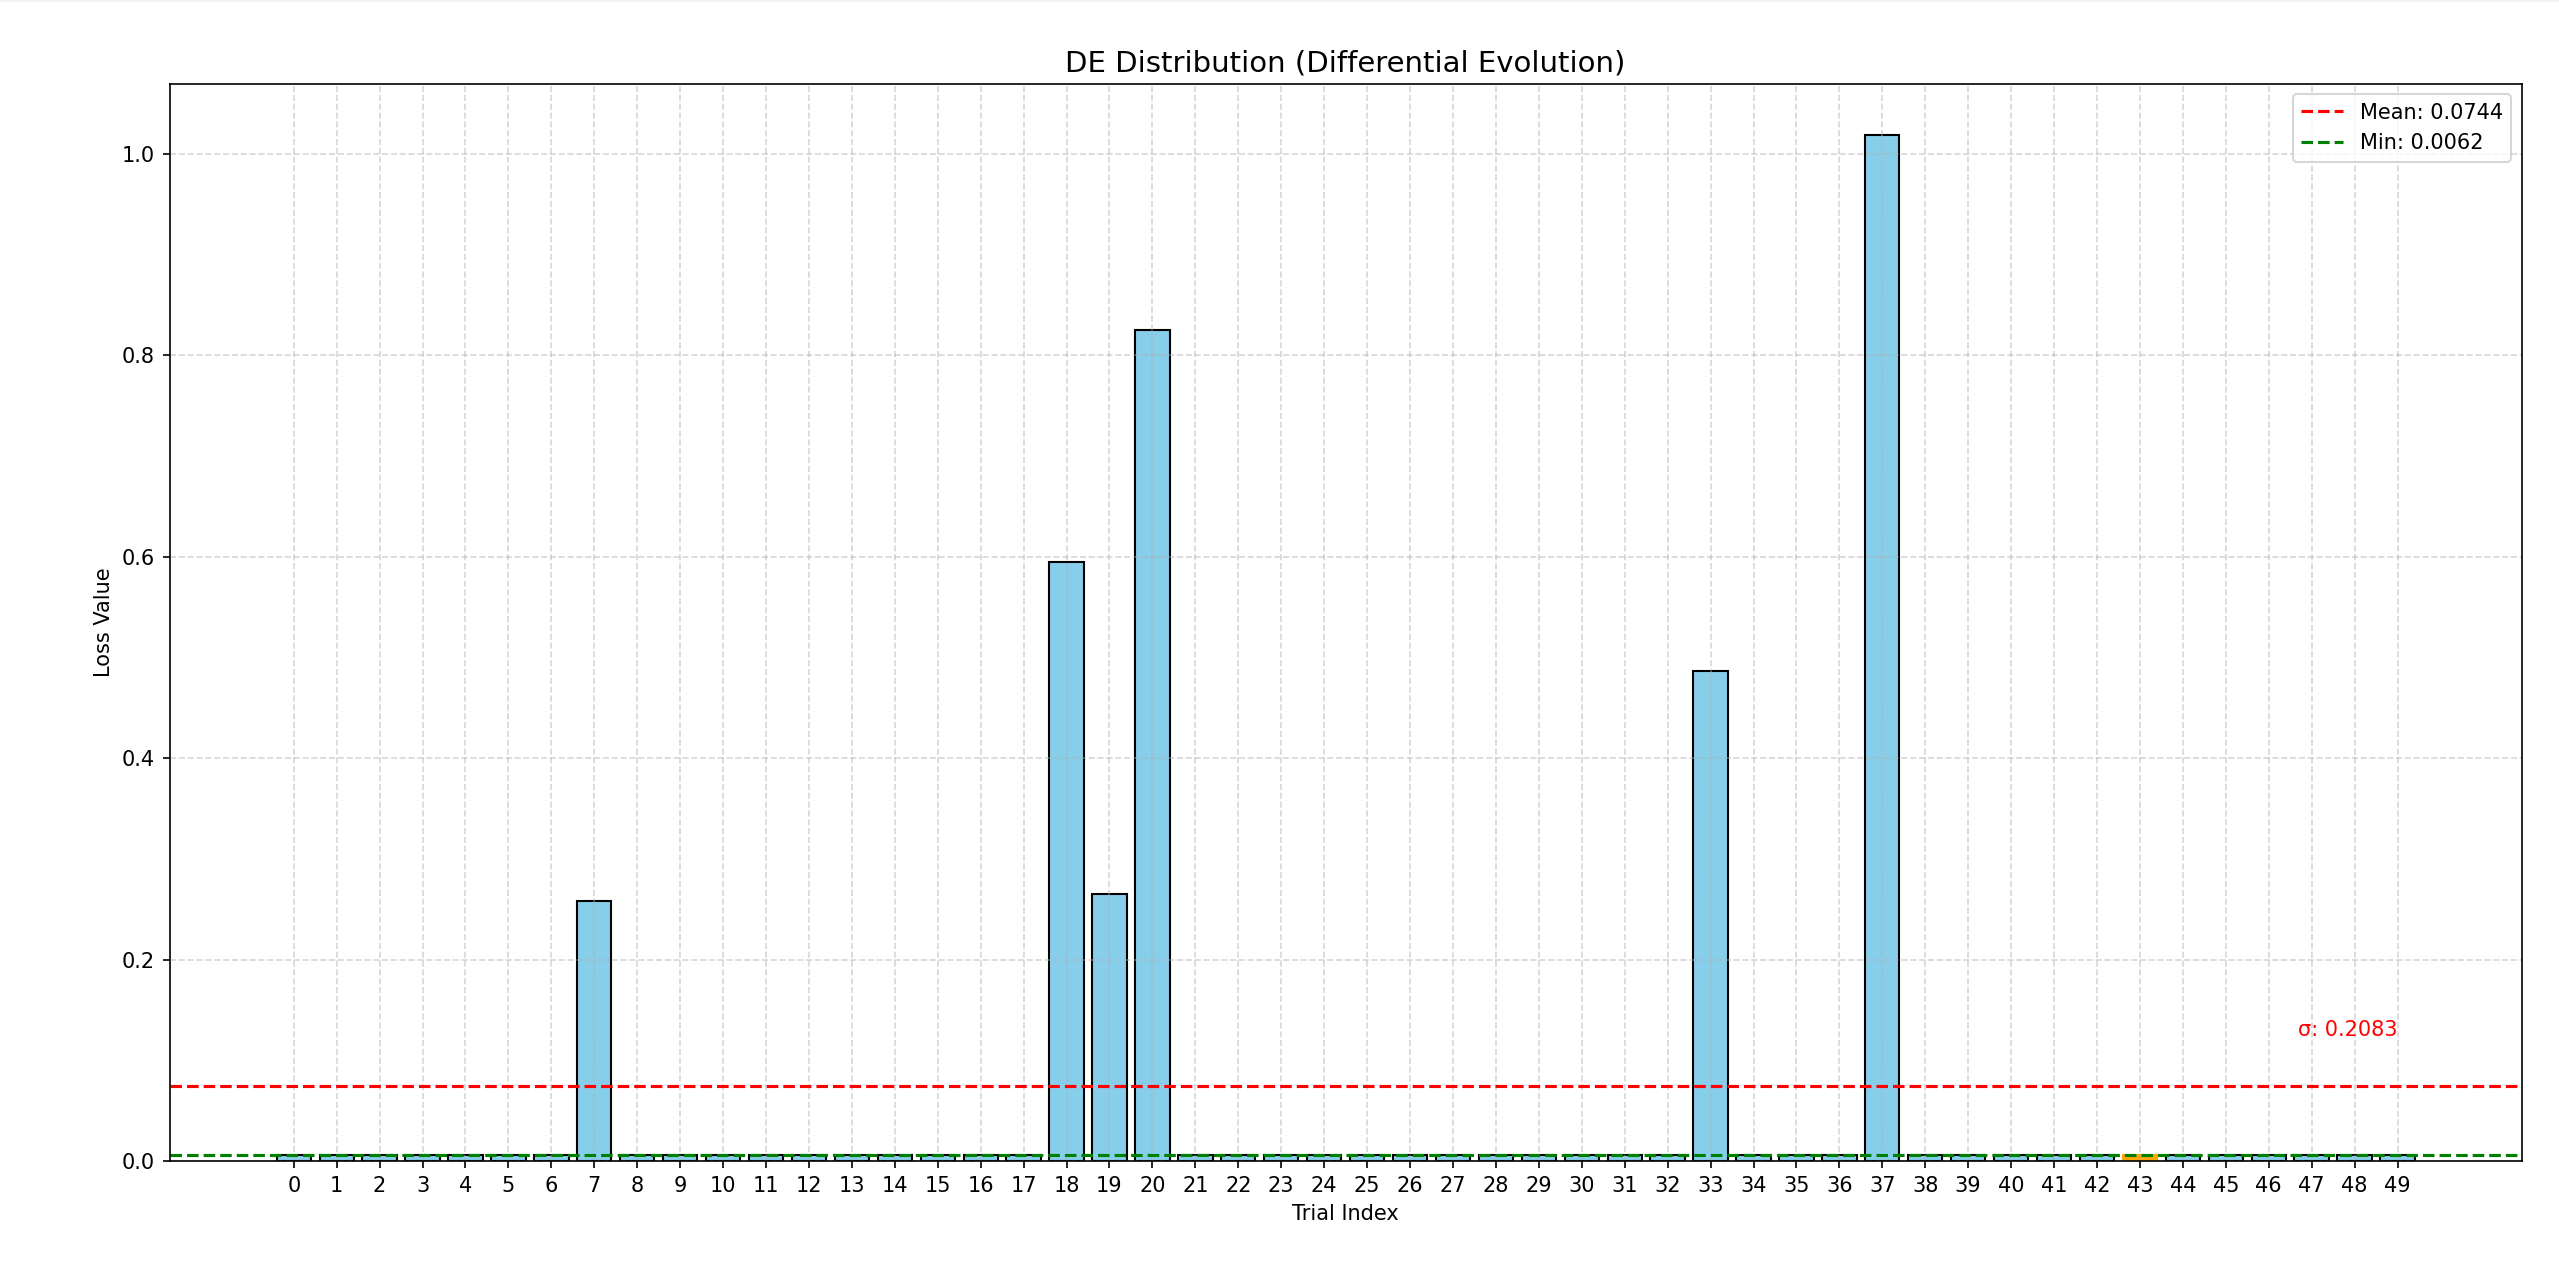
\includegraphics[width=1.0\columnwidth]{figures/DE2000.png}
\bicaption[50次独立优化实验柱状损失图]{50次独立优化实验柱状损失图。}[Histogram of loss values from 50 independent optimization experiments]{Histogram of loss values from 50 independent optimization experiments.}
\label{figure3: 柱状loss}
\end{figure}

\noindent\textbf{(2)色域覆盖度评估}

\circled{1} \textbf{色度空间三角形面积变化}

为评估映射后色域覆盖度变化,我们进一步对比了sRGB 色度三角与模型输出映射后所得的色度三角面积。面积通过三角形在 CIE xy 色度图上的顶点(RGB 基色经映射后的 xy 坐标)计算而得。结果表明,所有 50 次优化中,面积差绝对值均低于 0.001,说明映射后色域几乎无压缩,色彩覆盖极小损失。

\begin{figure}[h]
\centering
\captionsetup{font={small, stretch=1.312}}
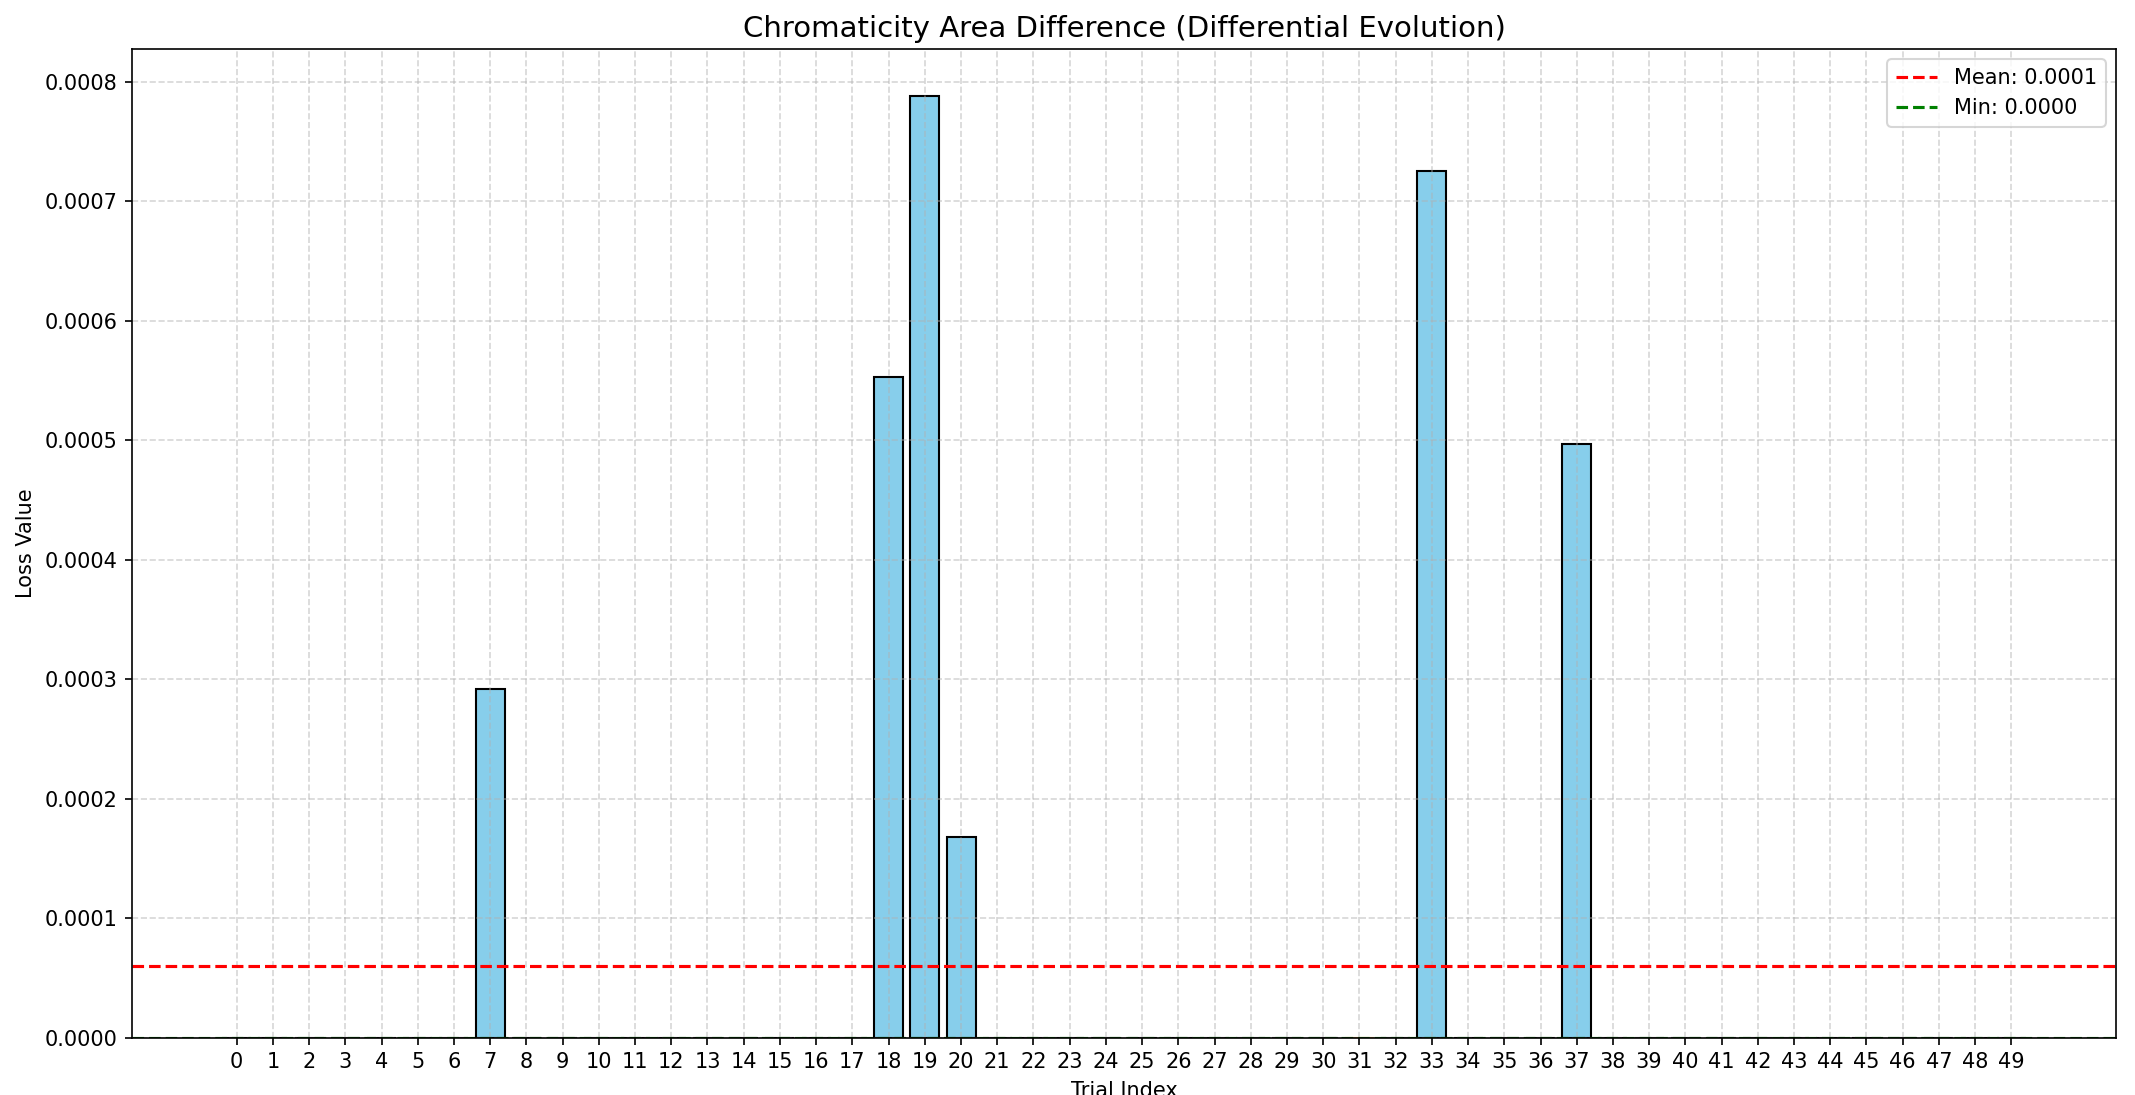
\includegraphics[width=0.8\columnwidth]{figures/面积Loss.png}
\bicaption[50次独立优化实验面积差图]{50次独立优化实验面积差图。}[Area difference plot from 50 independent optimization experiments]{Area difference plot from 50 independent optimization experiments.}
\label{figure3: 面积diff}
\end{figure}

显然我们可以得出,模型在保持色域范围完整性的同时,完成了精准的 RGB 空间映射,并且与 sRGB 的覆盖几乎一致,无明显压缩或扭曲现象。映射后的面积误差控制在 $10^{-3}$ 量级,说明模型不仅保持了色彩准确性,也很好地保留了 BT.2020 色域映射后的覆盖特性。

\circled{2} \textbf{色度图可视化对比}

为直观评估映射效果,我们将 BT.2020、sRGB 以及映射后所得色度三角同时绘制于 CIE 1931 xy 色度图中(见图 3)。可以观察到,模型优化后所得色度三角与标准 sRGB 色域几乎完全重合,进一步验证了在极低感知误差下,实现了对目标色域的高保真拟合。

\begin{figure}[h]
\centering
\captionsetup{font={small, stretch=1.312}}
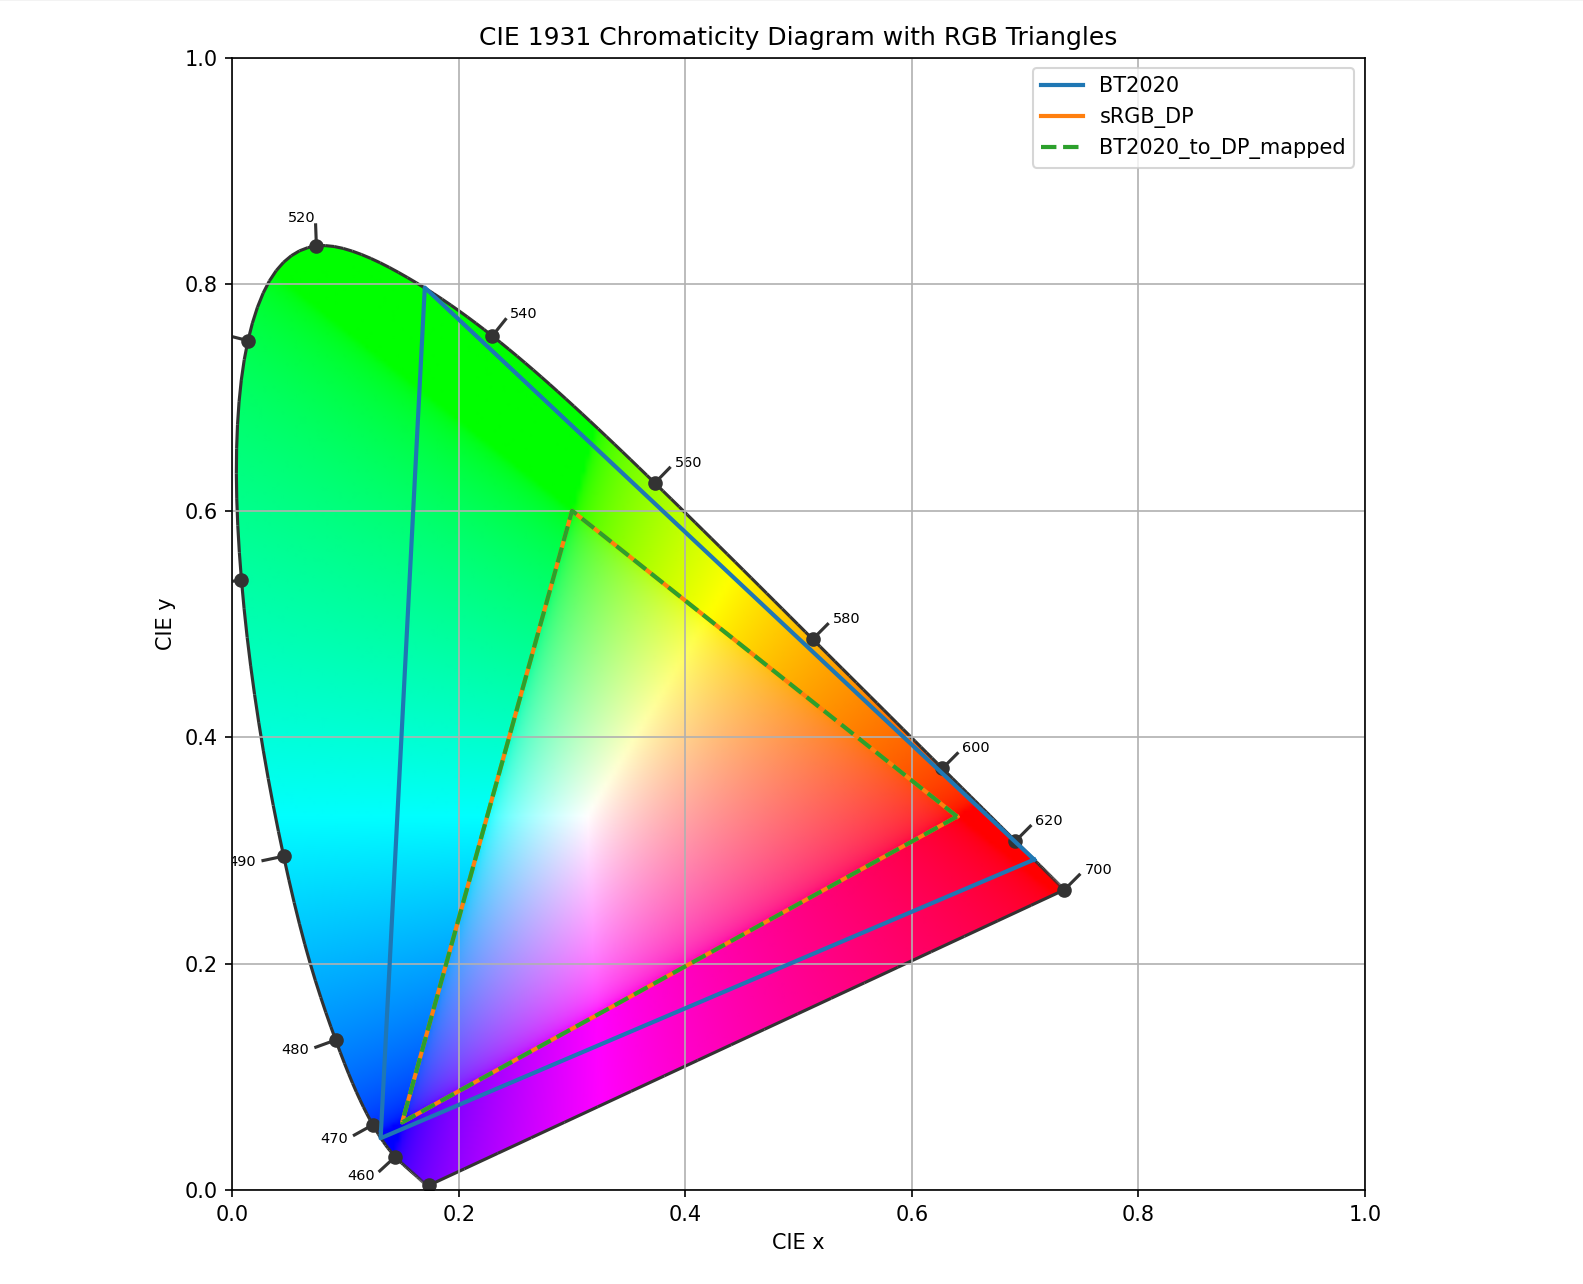
\includegraphics[width=0.8\columnwidth]{figures/色度.png}
\bicaption[色度图]{色度图。}[Chromaticity diagram]{Chromaticity diagram.}
\label{figure3: 色度图}
\end{figure}

\section[\hspace{-2pt}问题2:四通道到五通道颜色转换模型]{{\heiti\zihao{-3} \hspace{-8pt}问题2:四通道到五通道颜色转换模型}}\label{section3: 问题2:四通道到五通道颜色转换模型}

\subsection[\hspace{-2pt}问题分析与建模目标]{{\heiti\zihao{4} \hspace{-8pt}问题分析与建模目标}}\label{section2: 问题分析与建模目标}

本问题旨在解决从 4 通道相机 (RGBV) 到 5 通道 LED 显示屏 (RGBCX) 的颜色空间转换问题。其核心挑战在于:

\noindent\textbf{(1)问题挑战分析}

\circled{1} \textbf{通道数量不匹配}:输入是 4 维,输出是 5 维。这意味着简单的线性变换可能无法有效完成映射,且需要模型能够"创造"出多余的输出通道信息。

\circled{2} \textbf{非线性转换复杂性}:相机捕捉到的 RGBV 信号与显示屏所需的 RGBCX 信号之间通常存在复杂的非线性关系,这可能源于设备响应曲线、环境光照、传感器特性以及显示屏自身的物理特性。

\circled{3} \textbf{感知差异最小化要求}:转换后的颜色应尽可能保留原始颜色的人眼感知,即 $\Delta E_{2000}$ 应尽可能小。这是衡量颜色转换质量的关键指标,简单地最小化数值误差可能无法保证视觉效果。

因此,我们的建模目标是建立一个能够将 4 维相机输入(RGBV)映射到 5 维显示输出(RGBCX)的非线性模型,并以最小化颜色感知差异(即 $\Delta E_{2000}$)为主要优化目标,同时保证输出值在合理的物理范围内。

\subsection[\hspace{-2pt}神经网络模型设计]{{\heiti\zihao{4} \hspace{-8pt}神经网络模型设计}}\label{section2: 神经网络模型设计}

鉴于颜色空间转换的复杂非线性特性,以及输入输出维度不匹配的问题,我们选择使用前馈神经网络 (Feedforward Neural Network, FNN) 来作为主要的映射模型。

\noindent\textbf{(1)ColorNet架构设计}

我们设计了一个包含多个全连接层的神经网络,其结构如下:

\textbf{输入层}包含4个神经元,每个神经元对应相机捕捉到的一个颜色通道值:红(R)、绿(G)、蓝(B),以及额外的V通道(假设为某种光谱以外的特殊通道或相机特定校准通道)。输入数据直接传入,不进行激活函数处理。

\textbf{隐藏层架构}采用了3个隐藏层,以提供足够的模型容量来学习复杂的非线性映射。第一隐藏层将4维输入映射到64维特征空间,ReLU激活函数$f(x) = \max(0, x)$引入了非线性,使得网络能够学习到非线性特征。第二隐藏层进一步将特征维度提升至128维,增加维度有助于网络发现更丰富的特征组合。第三隐藏层将特征维度降回64维,这种"宽-窄"结构有助于信息在不同抽象层次上的流动和提炼。

\textbf{输出层}包含5个神经元,对应LED显示屏的五个输出通道:红(R)、绿(G)、蓝(B)、青(C),以及额外的X通道(假设为一种补充红色或特定效果通道)。Sigmoid激活函数$f(x) = \frac{1}{1+e^{-x}}$将输出值限制在[0,1]范围内,保证输出的物理合理性。

选择FNN的优势在于其灵活性和通用性。无需对输入输出关系进行复杂的先验假设,FNN可以通过训练自动从数据中学习到最佳的映射方式。多层结构和非线性激活函数使其能够处理高度复杂的颜色转换曲线和相互作用。

\subsection[\hspace{-2pt}损失函数设计]{{\heiti\zihao{4} \hspace{-8pt}损失函数设计}}\label{section2: 损失函数设计}

为了实现模型"最小化感知差异"的核心目标,我们设计了一个混合损失函数 (Combined Loss)。这个损失函数融合了两种不同的误差度量,旨在同时满足数值准确性和视觉准确性。

\noindent\textbf{(1)混合损失函数组成}

我们的混合损失函数由两个主要部分组成:

\textbf{均方误差损失(MSE)}定义为$ L_{MSE} = \frac{1}{N} \sum_{i=1}^N \| \text{pred\_rgbcx}_i - \text{target\_rgbcx}_i \|^2 $,其中$N$是样本数量,$\text{pred\_rgbcx}_i$是模型对第$i$个样本的5通道预测输出,$\text{target\_rgbcx}_i$是第$i$个样本的真实5通道目标输出。MSE是一种普遍使用的回归损失,它惩罚了预测值与目标值之间的数值差异,确保了模型在所有5个输出通道上的数值接近目标值,有助于网络的稳定训练,防止输出值出现极端或不合理的波动。

\textbf{感知误差损失($\Delta E_{2000}$)}定义为$ L_{\Delta E_{2000}} = \frac{1}{N} \sum_{i=1}^N \Delta E_{2000}(\text{pred\_lab}_i, \text{target\_lab}_i) $,这里$\text{pred\_lab}_i$是将模型预测的RGBCX输出中的RGB部分转换到Lab颜色空间的结果,而$\text{target\_lab}_i$则是将真实RGBCX目标中的RGB部分转换到Lab颜色空间的结果。转换过程包括:首先将sRGB空间下的RGB值转换为线性RGB值,然后通过3×3转换矩阵$M_{sRGB \to XYZ}$得到XYZ空间坐标;接着将XYZ坐标(经过白点归一化)转换为Lab坐标,这个转换涉及非线性函数$f(t)$,用于模拟人眼对亮度的非线性感知;最后使用PyTorch实现的$\Delta E_{2000}$公式计算预测Lab值与目标Lab值之间的颜色差异。

$L_{\Delta E_{2000}}$是本模型的核心创新点,因为它直接优化了人眼感知的颜色差异。相比于MSE仅关注数值上的匹配,$\Delta E_{2000}$损失能够引导模型生成在视觉上更接近目标颜色的输出。

\noindent\textbf{(2)损失函数权重平衡}

总损失函数定义为$ L_{total} = \alpha \cdot L_{MSE} + \beta \cdot L_{\Delta E_{2000}} $。在代码中,我们设置了$\alpha=0.1$和$\beta=1.0$。更高的$\beta$值(1.0)表明我们赋予$\Delta E_{2000}$损失更高的权重,明确指出我们优先考虑颜色转换的感知准确性。较低的$\alpha$值(0.1)虽然$\Delta E_{2000}$是主要目标,但保留一定比例的MSE损失仍然有益,可以提供一个更平滑的优化曲面。通过调整$\alpha$和$\beta$,可以在数值精确度和感知准确度之间找到最佳平衡点,这个平衡点通常需要根据具体的应用场景和视觉要求进行实验和调整。

\subsection[\hspace{-2pt}数据生成与训练策略]{{\heiti\zihao{4} \hspace{-8pt}数据生成与训练策略}}\label{section2: 数据生成与训练策略}

由于实际的 4 通道相机和 5 通道显示屏数据通常难以获取,我们采用了模拟数据生成的方法。

\noindent\textbf{(1)训练数据生成策略}

\circled{1} \textbf{输入数据生成}
\begin{itemize}
    \item 随机生成 $n_samples$ (例如 4000) 个样本,每个样本包含 4 个通道的值
    \item 每个通道的值都在 [0, 1] 范围内均匀随机分布
    \item 这模拟了相机在各种亮度(R, G, B)和特殊通道 (V) 下可能捕捉到的信号
\end{itemize}

\circled{2} \textbf{目标数据生成}
\begin{itemize}
    \item 目标数据的生成旨在模拟一个相对复杂但可控的真实世界颜色转换
    \item 首先,通过一个预设的线性变换矩阵 $W$ 对输入 $X$ 进行加权乘法,得到线性输出 $Y_{linear}$
    \item 接着,在 $Y_{linear}$ 的基础上添加一个非线性扰动,这个扰动项是基于输入 R 通道的一个正弦函数
    \item 最后,将所有输出值裁剪到 [0, 1] 范围,确保颜色通道值保持在物理上合理的范围内
\end{itemize}

\noindent\textbf{(2)模型训练策略}

我们采用了系统化的训练策略来确保模型的有效学习。在优化器选择方面,我们选用AdamW优化器,它是Adam优化器的一种改进版本,在权重衰减(L2正则化)的处理上更为有效,有助于防止过拟合。学习率设置为$5 \times 10^{-4}$,这个学习率是一个常用的起始值,它足够小以避免训练发散,又足够大以保证合理的收敛速度。

在数据处理方面,我们将生成的总数据集按80\%训练集和20\%验证集进行划分,训练集用于模型的参数更新,验证集用于在训练过程中评估模型的泛化能力。训练过程采用小批量(batch size=32)的方式进行,训练数据在每个epoch开始前会进行随机打乱,批次训练有助于提高训练效率、平滑梯度、防止过拟合。

在计算资源和监控方面,模型训练会优先使用GPU("cuda")如果可用,否则退回到CPU("cpu")。在训练过程中,每隔一定epoch会打印当前的训练损失和验证损失,以便实时监控模型的学习进度和性能。

通过上述详细的模型建立和解析,我们不仅明确了模型的基本架构和关键组成部分,更深入地探讨了其设计哲学和每个组件在解决颜色空间转换问题中的作用,尤其是混合损失函数在平衡数值和感知准确性方面的核心价值。

\subsection[\hspace{-2pt}模型求解和结果分析]{{\heiti\zihao{4} \hspace{-8pt}模型求解和结果分析}}\label{section2: 模型求解和结果分析}

\noindent\textbf{(1)训练过程分析}

\circled{1} \textbf{损失曲线分析}

通过运行提供的 Python 代码,我们训练了 ColorNet 模型。训练损失曲线展示了模型在训练集和验证集上的收敛情况。

\begin{figure}[H]
\centering
\captionsetup{font={small, stretch=1.312}}
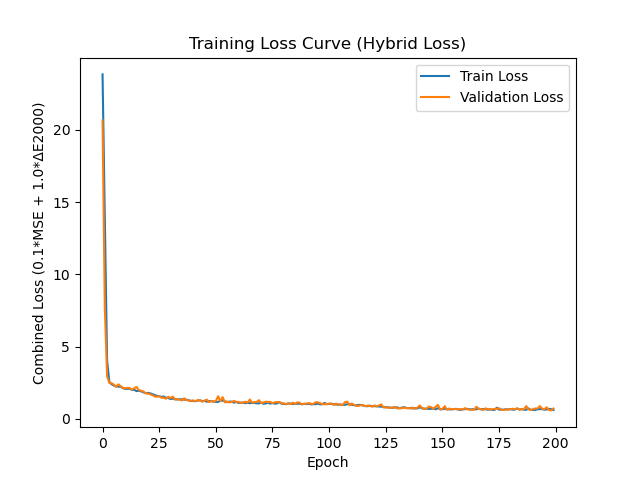
\includegraphics[width=0.8\columnwidth]{figures/Training_Loss_Curve.png}
\bicaption[训练损失曲线(混合损失)]{训练损失曲线(混合损失)。}[Training Loss Curve (Hybrid Loss)]{Training Loss Curve (Hybrid Loss).}
\label{figure2: loss_curve}
\end{figure}

从损失曲线可以看出,随着训练 epoch 的增加,训练损失和验证损失均呈现下降趋势,并最终趋于稳定。这表明模型成功地从模拟数据中学习到了 RGBV 到 RGBCX 的映射关系,且没有出现明显的过拟合现象。

\noindent\textbf{(2)感知性能评估}

为了更直观地评估模型的感知性能,我们计算了验证集上预测颜色与目标颜色之间的$\Delta E_{2000}$误差,并绘制了直方图和累积分布函数(CDF)。

\begin{figure}[H]
\centering
\captionsetup{font={small, stretch=1.312}}
\includegraphics[width=0.8\columnwidth]{figures/ΔE2000_Error_Histogram.png}
\bicaption[ΔE2000误差直方图(混合损失训练)]{ΔE2000误差直方图(混合损失训练)。}[ΔE2000 Error Histogram (Trained with Hybrid Loss)]{ΔE2000 Error Histogram (Trained with Hybrid Loss).}
\label{figure2: delta_e_histogram}
\end{figure}

\begin{figure}[H]
\centering
\captionsetup{font={small, stretch=1.312}}
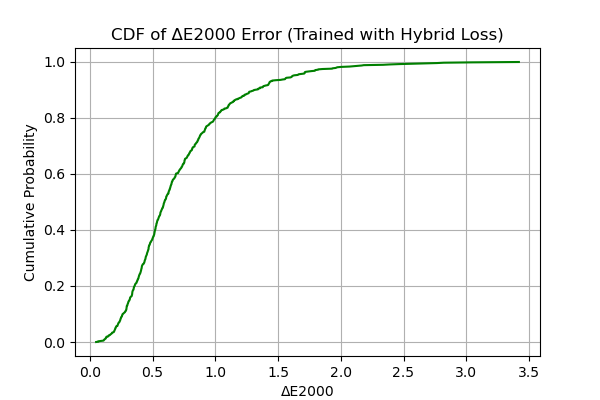
\includegraphics[width=0.8\columnwidth]{figures/CDF.png}
\bicaption[ΔE2000误差累积分布函数(混合损失训练)]{ΔE2000误差累积分布函数(混合损失训练)。}[CDF of ΔE2000 Error (Trained with Hybrid Loss)]{CDF of ΔE2000 Error (Trained with Hybrid Loss).}
\label{figure2: delta_e_cdf}
\end{figure}

从误差分析结果可以看出,直方图显示了$\Delta E_{2000}$误差的分布情况,大部分预测颜色的$\Delta E_{2000}$值集中在较低的范围内(例如0-2之间),这意味着模型能够很好地重现大部分目标颜色。CDF图更清晰地展示了误差的累积分布,通常认为$\Delta E_{2000} < 1.0$表示人眼难以察觉的颜色差异,$\Delta E_{2000} < 2.0-3.0$表示可接受的颜色差异。

\noindent\textbf{(3)色域可视化分析}

为了理解4通道输入系统和5通道输出系统各自的色域以及它们之间的关系,我们在CIE 1931色度图上绘制了它们的基色坐标点和由这些基色围成的色域(多边形)。

\begin{figure}[H]
\centering
\captionsetup{font={small, stretch=1.312}}
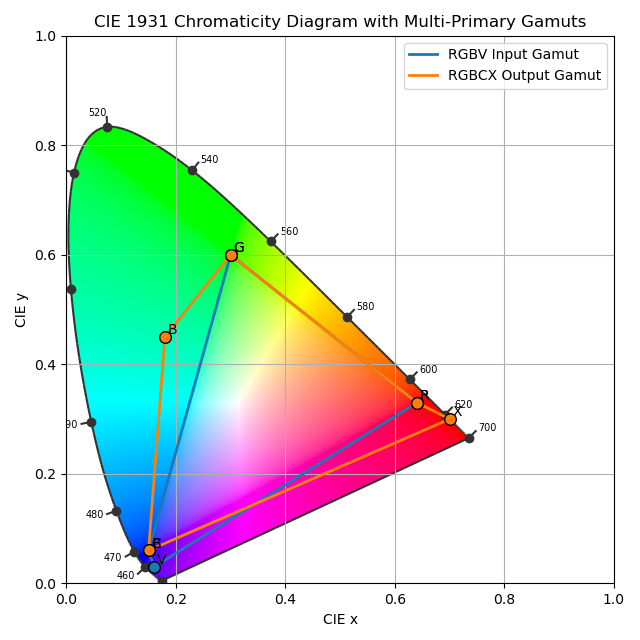
\includegraphics[width=0.67\columnwidth]{figures/色度图.png}
\bicaption[CIE 1931色度图与多基色色域]{CIE 1931色度图与多基色色域。}[CIE 1931 Chromaticity Diagram with Multi-Primary Gamuts]{CIE 1931 Chromaticity Diagram with Multi-Primary Gamuts.}
\label{figure2: chromaticity_diagram}
\end{figure}

从色域分析结果可以看出,输入色域(RGBV Input Gamut)由sRGB的R、G、B三原色以及新增的'V'(紫色)通道构成,由于'V'通道的加入,相机色域在蓝色-紫色区域得到一定的扩展。输出色域(RGBCX Output Gamut)由sRGB的R、G、B三原色,以及新增的'C'(青色)和'X'(假设更深的红色)通道构成,通过'C'和'X'的加入,显示屏的色域在蓝绿色和红色区域相对于传统sRGB显示屏得到了显著扩展。五通道显示屏的色域明显大于四通道相机的色域,这为颜色转换提供了更大的灵活性和再现能力。

\noindent\textbf{(4)样本预测效果}

为了直观地展示模型对具体颜色样本的转换效果,我们随机选择了几个验证集样本,并将其原始输入、目标输出和模型预测输出进行并排可视化。

\begin{figure}[H]
\centering
\captionsetup{font={small, stretch=1.312}}
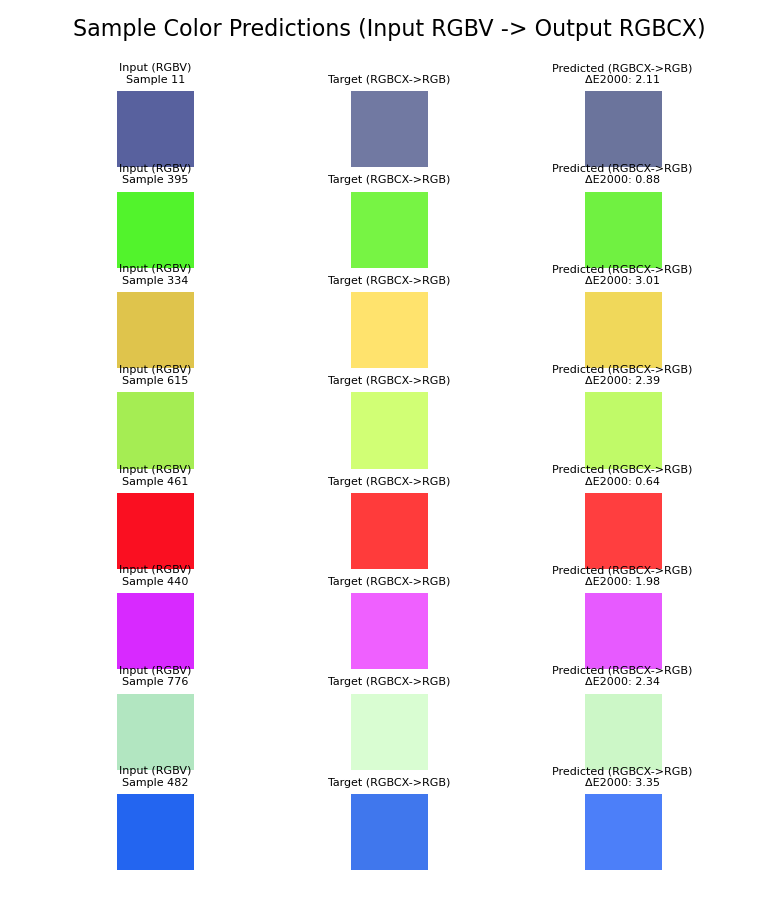
\includegraphics[width=0.8\columnwidth]{figures/Sample.png}
\bicaption[样本颜色预测(输入RGBV→输出RGBCX)]{样本颜色预测(输入RGBV→输出RGBCX)。}[Sample Color Predictions (Input RGBV → Output RGBCX)]{Sample Color Predictions (Input RGBV → Output RGBCX).}
\label{figure2: sample_predictions}
\end{figure}

每行代表一个样本:Input(RGBV)列显示了原始相机输入通过简化映射到RGB的颜色,代表了相机"看到"的颜色;Target(RGBCX->RGB)列显示了目标5通道输出通过简化映射到RGB的颜色,代表了理想情况下显示屏应该呈现的颜色;Predicted(RGBCX->RGB)列显示了模型预测的5通道输出通过简化映射到RGB的颜色,并标注了与目标颜色的$\Delta E_{2000}$误差。通过对比可以看到,绝大多数样本的预测颜色与目标颜色非常接近,且$\Delta E_{2000}$值较低,进一步验证了模型的有效性。

\section[\hspace{-2pt}问题3:LED显示器颜色校正模型]{{\heiti\zihao{-3} \hspace{-8pt}问题3:LED显示器颜色校正模型}}\label{section4: 问题3:LED显示器颜色校正模型}

LED显示器在实际应用中存在颜色失真问题,测量值与目标值之间存在显著偏差。本节基于CIE Lab色彩空间和三基色原理,建立了一个结合伽马校正与线性矩阵变换的颜色校正模型,通过差分进化算法优化校正参数,实现精确的颜色还原。

\subsection[\hspace{-2pt}模型建立流程]{{\heiti\zihao{4}\hspace{-8pt}模型建立流程}}\label{subsec:3-model-build}

\noindent \textbf{(1)变量定义}

\circled{1} \textbf{线性 RGB 向量}
\begin{equation}
  \mathbf{x}=\begin{bmatrix}R_\ell\\G_\ell\\B_\ell\end{bmatrix}\in[0,1]^3.
\end{equation}
其中$R_\ell, G_\ell, B_\ell$分别表示经过反伽马校正后的线性RGB分量。

\circled{2} \textbf{校正参数}
\begin{align}
  M &\in\mathbb{R}^{3\times3}, \quad \text{(校正变换矩阵)}\\
  \mathbf{b} &\in\mathbb{R}^3. \quad \text{(偏置向量)}
\end{align}

\circled{3} \textbf{校正映射}
\begin{equation}
  \mathbf{y}=\mathrm{clip}\!\bigl(M\mathbf{x}+\mathbf{b},[0,1]\bigr).
\end{equation}
该映射确保输出值域限制在有效的RGB范围内。

\noindent\textbf{(2)伽马校正模型}

基于第\ref{chapter3: 理论基础}章中建立的伽马校正理论(见第\ref{section2: 伽马校正理论}节),对每个颜色通道$c \in \{R,G,B\}$,建立响应关系:
\begin{equation}
  I_{\text{meas},c} = S_c \cdot (I_{\text{target},c})^{\gamma_c}
\end{equation}
其中$\gamma_c$为伽马值,$S_c$为比例因子。

通过对三种基色图像的实际测量数据进行伽马参数估计,采用对数线性回归方法(详见第\ref{subsection2: 伽马参数估计}节),得到的结果如表\ref{table:gamma_params}所示:

\begin{table}[h!]
\small    % 设置表格字体为5号
\setstretch{1.245}        % 设置具有指定弹力的橡皮长度(原行宽的1.2倍)
\captionsetup{font={small, stretch=1.512}}
\centering
\bicaption[不同基色图像的伽马参数估计结果]{不同基色图像的伽马参数估计结果。}[Gamma parameter estimation results for different primary color images]{Gamma parameter estimation results for different primary color images.}    % 中英文标题
\begin{tabularx}{\textwidth}{lCCCCCC}
\toprule
\multirow{2}{*}{图像类型} & \multicolumn{3}{c}{伽马值 ($\gamma_c$)} & \multicolumn{3}{c}{比例因子 ($S_c$)} \\
\cline{2-7}
 & \raisebox{-2pt}{R通道} & \raisebox{-2pt}{G通道} & \raisebox{-2pt}{B通道} & \raisebox{-2pt}{R通道} & \raisebox{-2pt}{G通道} & \raisebox{-2pt}{B通道} \\
\midrule
红色图像 & 0.022 & 0.229 & 0.230 & 0.862 & 0.988 & 0.988 \\
绿色图像 & 0.228 & 0.022 & 0.232 & 0.988 & 0.862 & 0.987 \\
蓝色图像 & 0.231 & 0.228 & 0.022 & 0.988 & 0.988 & 0.861 \\
\bottomrule
\end{tabularx}
%\vspace{-20pt}
\label{table:gamma_params}
\end{table}

从伽马参数估计结果可以观察到一个重要现象:主色通道(红色图像的R通道、绿色图像的G通道、蓝色图像的B通道)的伽马值显著较小(约0.022),而非主色通道的伽马值相对较大(约0.23)。这表明LED显示器在显示主色时存在更强的非线性响应特性,需要更大的校正幅度。

根据第\ref{subsection2: 伽马校正变换}节中的伽马校正变换公式,线性化变换为:
\begin{align}
  \text{前向:} \quad &I_{\text{out}} = \text{clip}((I_{\text{in}} \cdot S)^{\gamma}, [0,1])\\
  \text{反向:} \quad &I_{\text{out}} = \text{clip}((I_{\text{in}})^{1/\gamma} / S, [0,1])
\end{align}

\noindent\textbf{(3)目标函数设计}

我们设计了一个综合的目标函数,包含多个组成部分以确保校正效果的全面性。

首先是色差损失,基于第\ref{section2: CIEDE2000色差公式}节中的CIE $\Delta E_{00}$色差公式构建目标函数:
\begin{equation}
L_{\mathrm{DE}}=\frac{1}{N}\sum_{k=1}^N \Delta E_{00}\!\bigl(\mathbf{L}_{\mathrm{t},k},\mathbf{L}_{\mathrm{c},k}\bigr)
\end{equation}
其中$\mathbf{L}_{\mathrm{t},k}$和$\mathbf{L}_{\mathrm{c},k}$分别表示第$k$个像素点的目标和校正后的CIE Lab值(Lab空间转换详见第\ref{section2: CIELab颜色空间}节)。

其次是正则化项:
\begin{equation}
L_{\mathrm{reg}}=\lambda_1\|M-I_3\|_F^2+\lambda_2\|\mathbf{b}\|_2^2
\end{equation}
用于防止校正矩阵过度偏离单位矩阵,确保变换的稳定性。

同时引入行列式惩罚:
\begin{equation}
L_{\det}=\lambda_3 \cdot \mathbf{1}\bigl(\det M\leq0 \lor |\det M|<\epsilon\bigr)
\end{equation}
其中$\epsilon=0.1$,确保变换矩阵的可逆性和数值稳定性。

最终的总目标函数为:
\begin{equation}
\mathcal{L}(M,\mathbf{b})=L_{\mathrm{DE}}+L_{\mathrm{reg}}+L_{\det}
\end{equation}
参数设置为$\lambda_1=\lambda_2=0.001$,$\lambda_3=1000$。

该目标函数综合考虑了颜色感知准确性、数值稳定性和矩阵可逆性,其中RGB到XYZ到Lab的完整转换流程详见第\ref{section2: CIEXYZ颜色空间}节和第\ref{section2: CIELab颜色空间}节。

\subsection[\hspace{-2pt}模型求解策略]{{\heiti\zihao{4}\hspace{-8pt}模型求解策略}}\label{subsec:3-solver}

考虑到目标函数的非凸性和多模态特征,采用全局-局部混合优化策略:

\noindent\textbf{(1)差分进化全局搜索}

\circled{1} \textbf{参数空间设定}

在参数空间$\{M_{ij}\in[-2,2],\,b_i\in[-0.1,0.1]\}$内进行全局搜索:
\begin{align}
  \text{种群大小:} &\quad \text{popsize} = 15\\
  \text{最大迭代:} &\quad \text{maxiter} = 200\\
  \text{变异因子:} &\quad F \in [0.5, 2.0]\\
  \text{交叉概率:} &\quad CR = 0.7
\end{align}
得到初值$\theta_0=(\operatorname{vec}(M_0),\mathbf{b}_0)$。

\circled{2} \textbf{差分进化操作}

通过经典的种群初始化、变异、交叉及选择等核心操作,DE算法能够迭代地搜寻旨在最小化以 $\Delta E_{00}$ 度量的感知色彩差异的解。

\noindent\textbf{(2)L-BFGS-B局部精调}

\circled{1} \textbf{局部优化设置}

以$\theta_0$为起点,采用拟牛顿法进行局部优化:
\begin{equation}
  (M^*,\mathbf{b}^*) = \arg\min_{M,\mathbf{b}} \mathcal{L}(M,\mathbf{b})
\end{equation}
\begin{align}
  \text{最大迭代:} &\quad 500\\
  \text{收敛容差:} &\quad 10^{-6}\\
  \text{梯度容差:} &\quad 10^{-5}
\end{align}

\noindent\textbf{(3)算法流程}

\circled{1} \textbf{完整算法描述}

\begin{algorithm}[H]\small
\setstretch{1.245} %设置具有指定弹力的橡皮长度(原行宽的1.2倍)
\renewcommand{\algorithmcfname}{算法}
	\caption{LED颜色校正算法}
	\KwIn{测量数据$\mathbf{X}_{\text{meas}} \in \mathbb{R}^{H \times W \times 3}$,目标数据$\mathbf{X}_{\text{target}} \in \mathbb{R}^{H \times W \times 3}$}
	\KwOut{校正矩阵$M^*$,偏置向量$\mathbf{b}^*$}
	
	\textbf{步骤1:伽马参数估计}\\
	\For{$c \in \{R,G,B\}$}{
		提取通道数据:$I_{\text{meas},c}$, $I_{\text{target},c}$\\
		拟合:$\log(I_{\text{meas},c}) = \gamma_c \log(I_{\text{target},c}) + \log(S_c)$\\
		求解:$\gamma_c$, $S_c$\\
	}
	
	\textbf{步骤2:数据预处理}\\
	反伽马校正:$\mathbf{X}_{\text{meas,lin}} \leftarrow \Gamma^{-1}(\mathbf{X}_{\text{meas}})$\\
	反伽马校正:$\mathbf{X}_{\text{target,lin}} \leftarrow \Gamma^{-1}(\mathbf{X}_{\text{target}})$\\
	
	\textbf{步骤3:全局优化}\\
	初始化DE种群:$\mathcal{P}_0 = \{\theta_1, \theta_2, \ldots, \theta_{\text{popsize}}\}$\\
	\For{$t = 1$ \textbf{to} $\text{maxiter}$}{
		\For{每个个体$\theta_i \in \mathcal{P}_t$}{
			变异:$\mathbf{v}_i = \theta_{r1} + F \cdot (\theta_{r2} - \theta_{r3})$\\
			交叉:$\mathbf{u}_i = \text{crossover}(\theta_i, \mathbf{v}_i, CR)$\\
			选择:$\theta_i^{t+1} = \arg\min_{\{\theta_i, \mathbf{u}_i\}} \mathcal{L}(\cdot)$\\
		}
	}
	获得最优个体:$\theta_0 = \arg\min_{\theta \in \mathcal{P}_{\text{final}}} \mathcal{L}(\theta)$\\
	
	\textbf{步骤4:局部精调}\\
	$(M^*, \mathbf{b}^*) \leftarrow \text{L-BFGS-B}(\theta_0, \mathcal{L})$\\
	
	\label{algorithm:led_correction}
\end{algorithm}
\vspace{20pt}

\noindent\textbf{(4)校正应用流程}

完整的颜色校正应用流程包括三个主要步骤:首先对输入sRGB进行反伽马校正,即线性化处理$\mathbf{x}_\ell = \Gamma^{-1}(\mathbf{x}_{\mathrm{srgb}})$;然后应用校正矩阵和偏置进行线性变换$\mathbf{y}_\ell = \mathrm{clip}\!\bigl(M^*\mathbf{x}_\ell+\mathbf{b}^*,[0,1]\bigr)$;最后进行正向伽马校正,重新编码恢复到sRGB空间$\mathbf{y}_{\mathrm{srgb}}=\Gamma(\mathbf{y}_\ell)$。

\subsection[\hspace{-2pt}模型验证与分析]{{\heiti\zihao{4}\hspace{-8pt}模型验证与分析}}\label{subsec:3-validation}

\noindent\textbf{(1)可视化结果分析}

\circled{1} \textbf{RGB通道校正对比}

\begin{figure}[H]
  \centering
  \captionsetup{font={small, stretch=1.312}}

  \begin{subfigure}[b]{0.6\textwidth}
    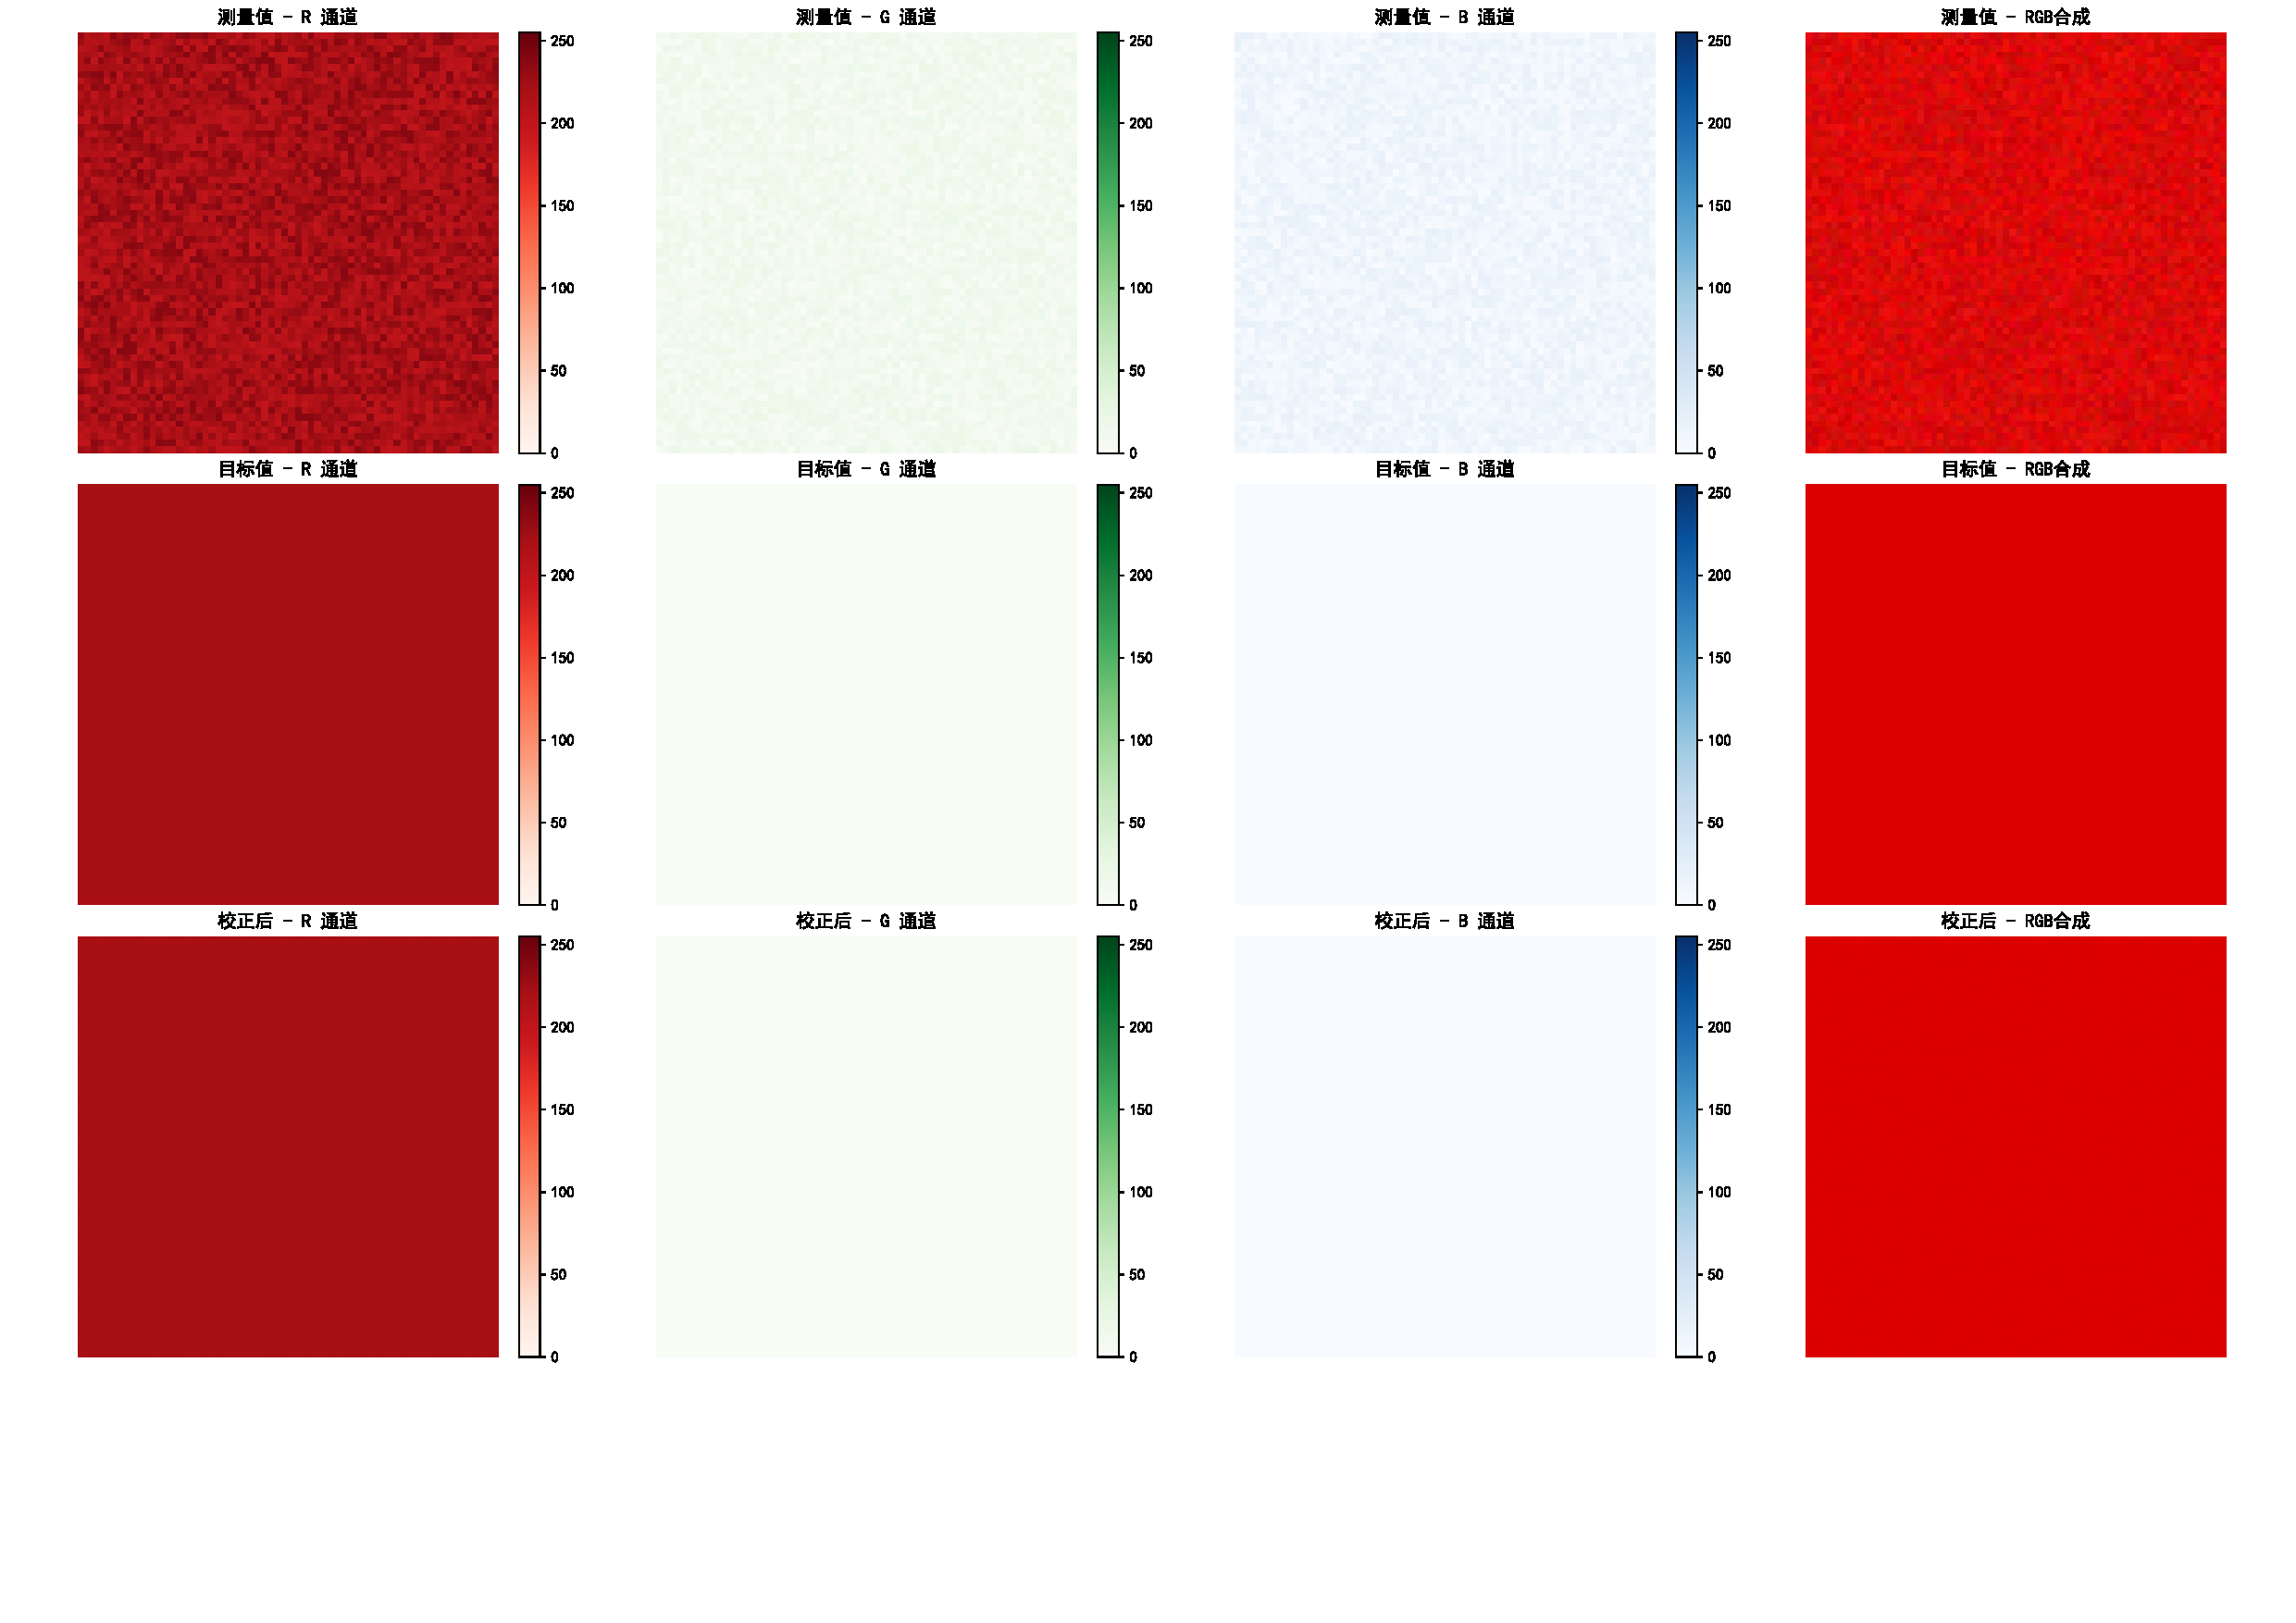
\includegraphics[width=\textwidth]{figures/model_solution/p3/R.pdf}
    \bicaption[红色图片各通道校正前后对比示意图]
        {红色图片各通道校正前后对比示意图。}[Comparison of pre- and post-correction for red image channels]{Comparison of pre- and post-correction for red image channels.}
    \label{figure4:r_compare}
  \end{subfigure}
  \hfill
  \begin{subfigure}[b]{0.6\textwidth}
    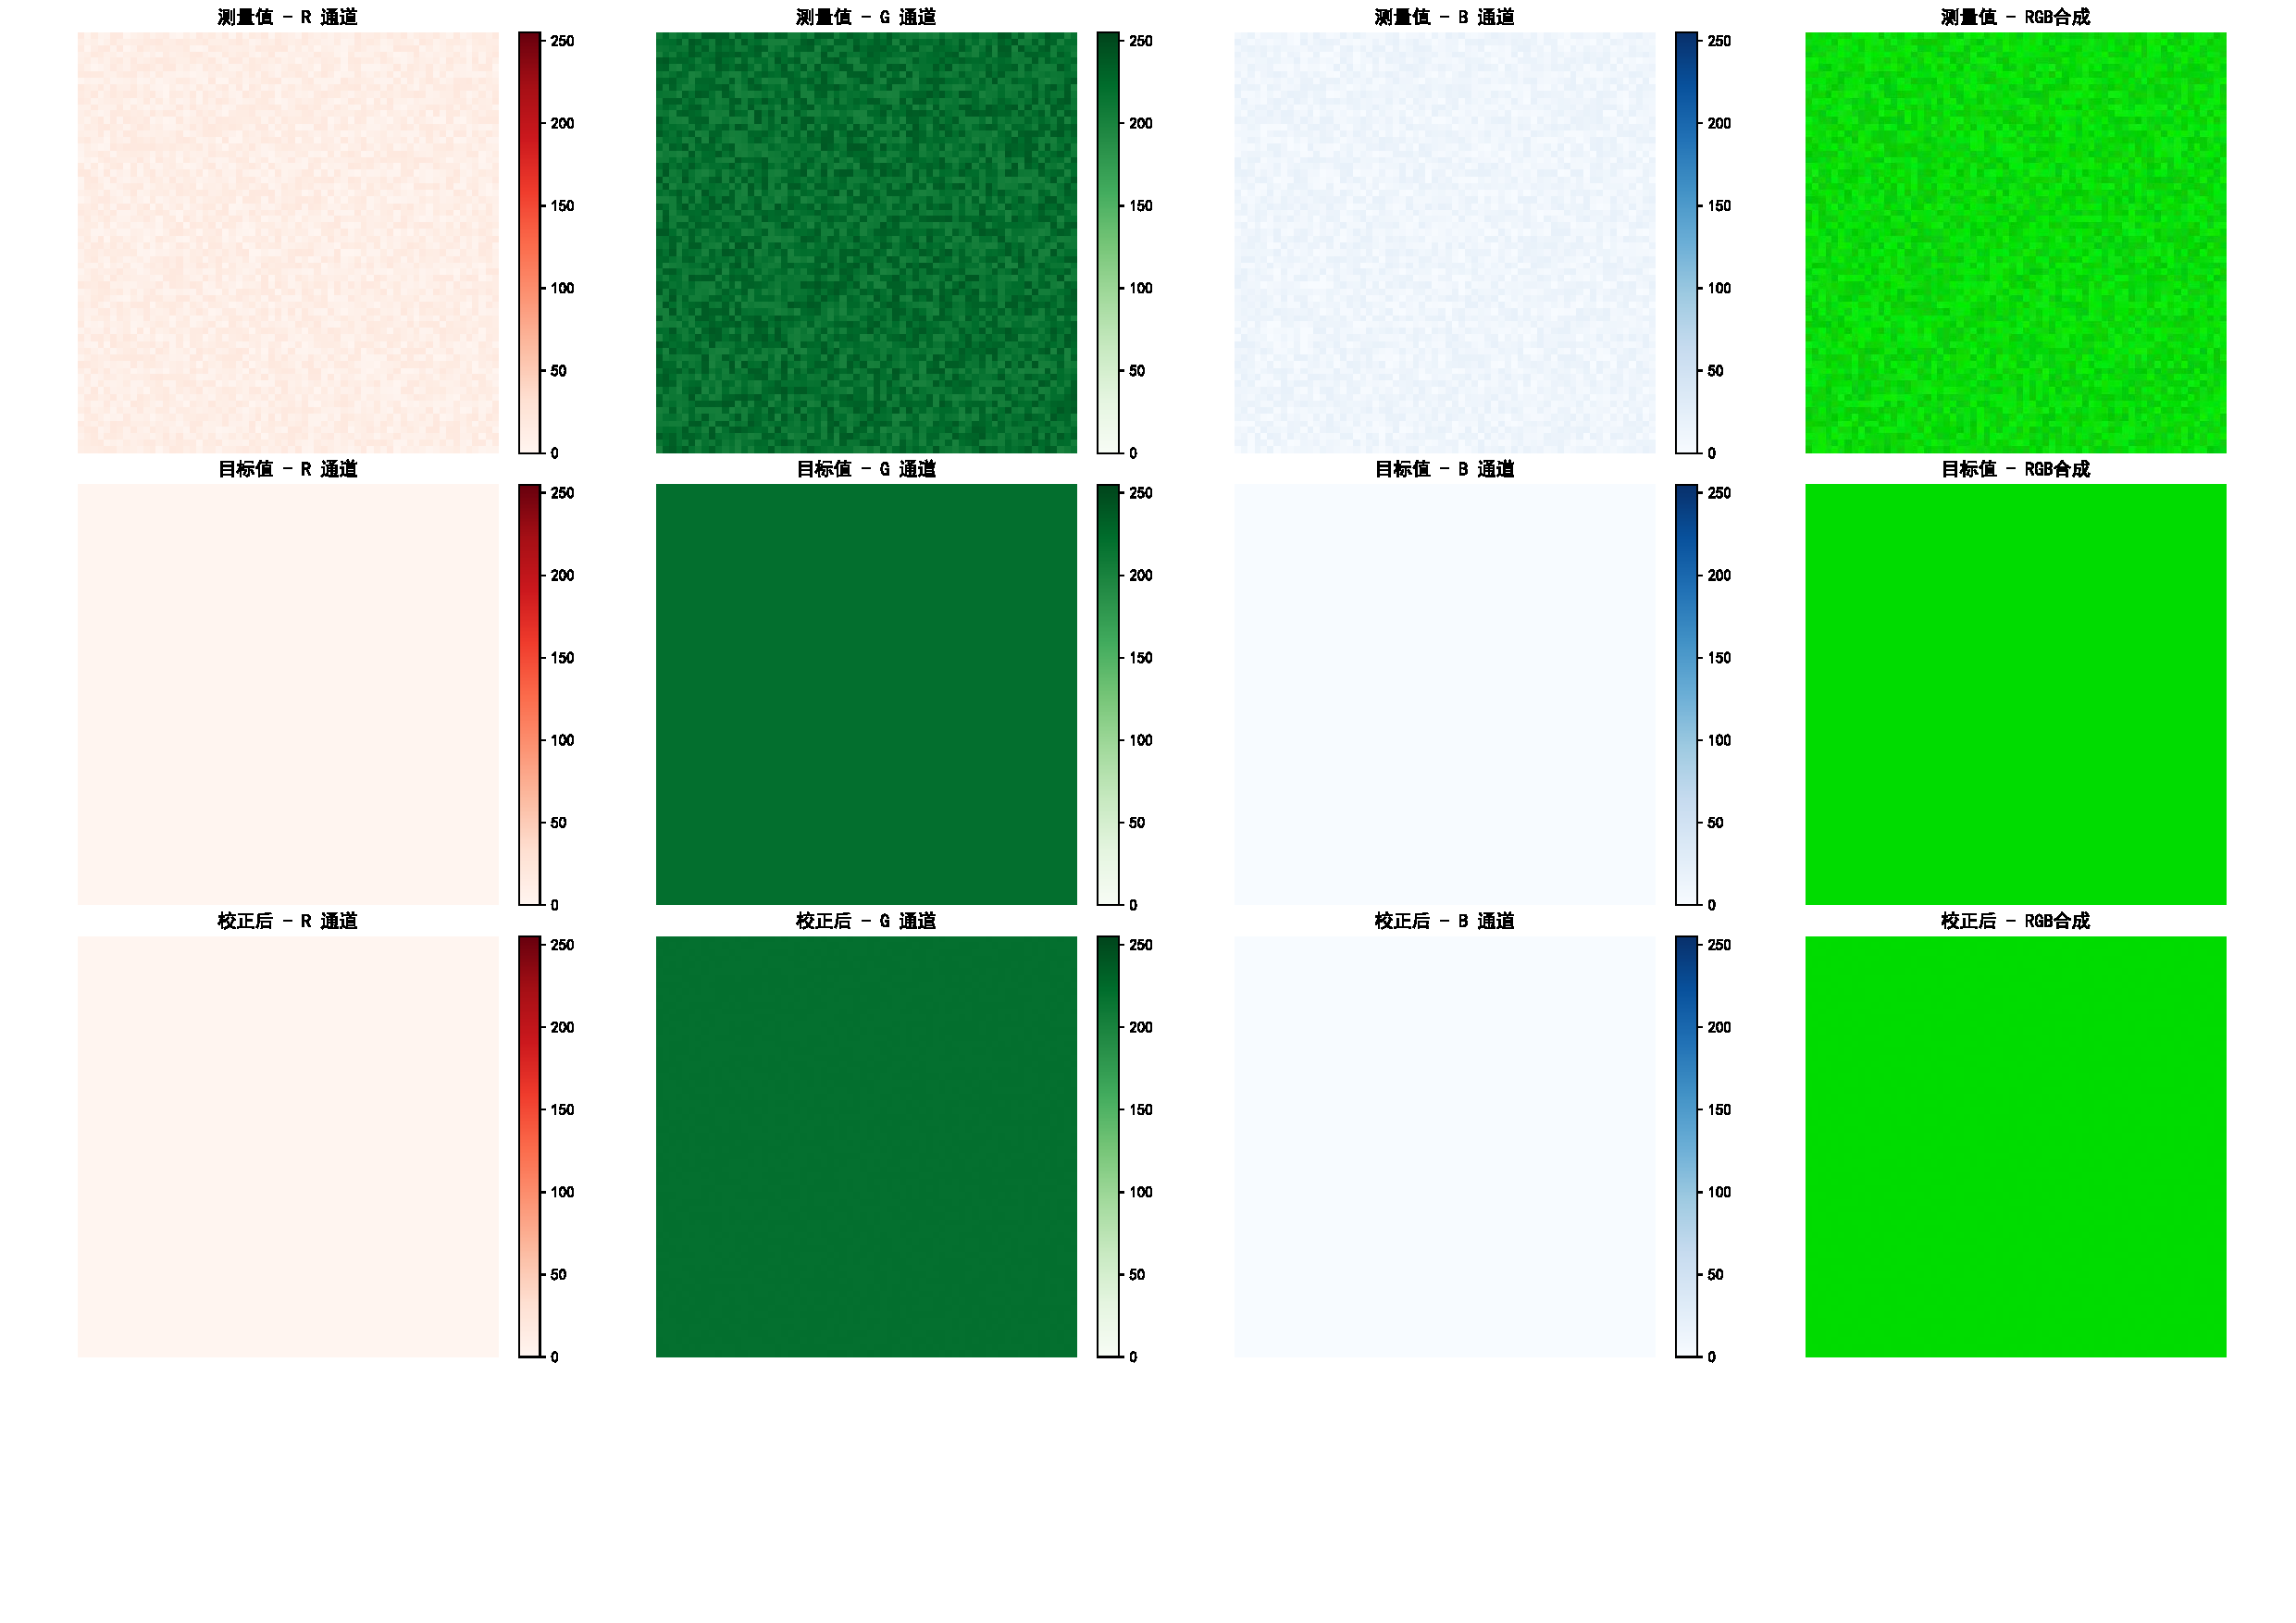
\includegraphics[width=\textwidth]{figures/model_solution/p3/G.pdf}
    \bicaption[绿色图片各通道校正前后对比示意图]
        {绿色图片各通道校正前后对比示意图。}[Comparison of pre- and post-correction for green image channels]{Comparison of pre- and post-correction for green image channels.}
    \label{figure4:g_compare}
  \end{subfigure}
  \hfill
  \begin{subfigure}[b]{0.6\textwidth}
    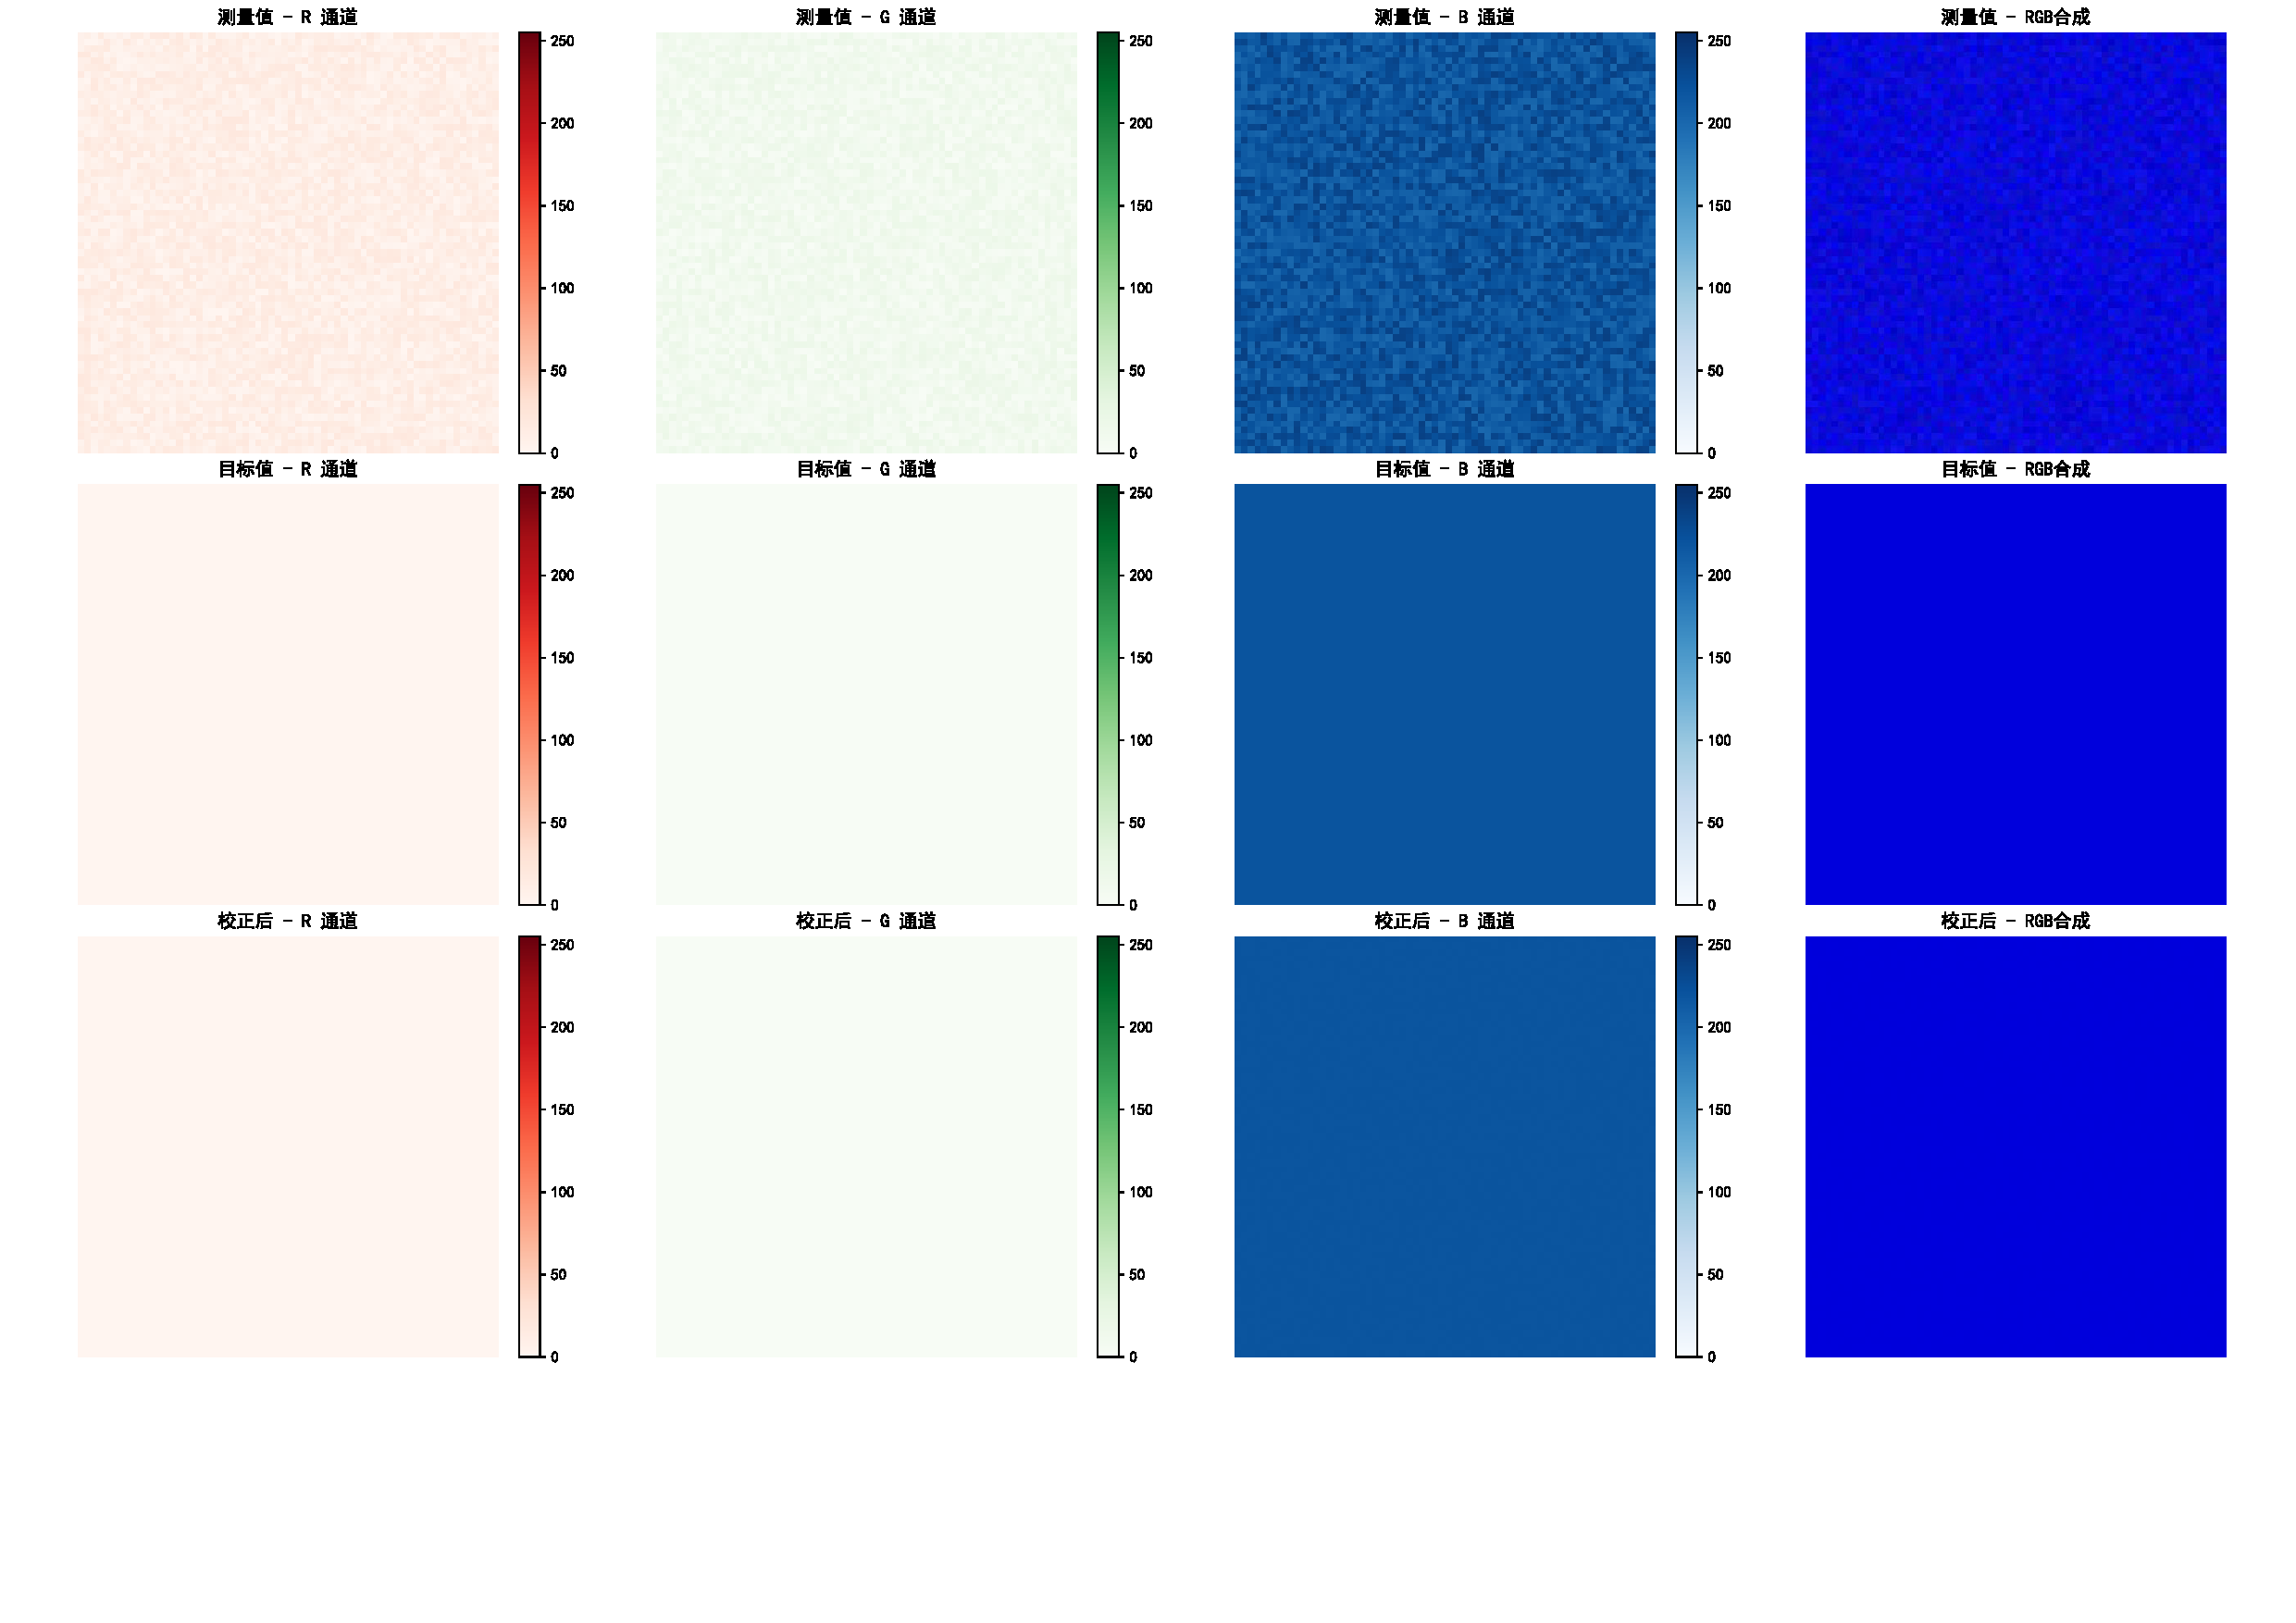
\includegraphics[width=\textwidth]{figures/model_solution/p3/B.pdf}
    \bicaption[蓝色图片各通道校正前后对比示意图]
        {蓝色图片各通道校正前后对比示意图。}[Comparison of pre- and post-correction for blue image channels]{Comparison of pre- and post-correction for blue image channels.}
    \label{figure4:b_compare}
  \end{subfigure}

  \bicaption[RGB三原色图像校正前后对比示意图]{RGB三原色图像校正前后对比示意图。}[Comparison of Pre- and Post-Correction for RGB Channels]{Comparison of Pre- and Post-Correction for RGB Channels.}
  \label{figure4:rgb_compare}
\end{figure}

通过可视化分析可以观察到,校正后的图像在色彩还原度和视觉效果方面均有显著改善,RGB各通道的分布更接近目标值。

\noindent\textbf{(2)定量评估结果}

基于CIE $\Delta E_{00}$色差评估标准,我们对三种基色图像(红色、绿色、蓝色)分别进行了颜色校正实验。表\ref{table:correction_results}展示了详细的定量评估结果。

\begin{table}[h!]
\small    % 设置表格字体为5号
\setstretch{1.245}        % 设置具有指定弹力的橡皮长度(原行宽的1.2倍)
\captionsetup{font={small, stretch=1.512}}
\centering
\bicaption[LED颜色校正效果定量评估结果]{LED颜色校正效果定量评估结果。}[Quantitative evaluation results of LED color correction]{Quantitative evaluation results of LED color correction.}    % 中英文标题
\begin{tabularx}{\textwidth}{lCCCC}
\toprule
评估指标 & 红色图像 & 绿色图像 & 蓝色图像 & 平均值 \\
\midrule
校正前平均色差 $\overline{\Delta E}_{00}^{\text{before}}$ & 2.540 & 2.418 & 1.519 & 2.159 \\
校正后平均色差 $\overline{\Delta E}_{00}^{\text{after}}$ & 0.106 & 0.115 & 0.063 & 0.095 \\
色差改善值 & 2.434 & 2.303 & 1.456 & 2.064 \\
改善百分比 & 95.8\% & 95.2\% & 95.9\% & 95.6\% \\
校正前最大色差 & 5.207 & 5.015 & 3.344 & 4.522 \\
校正后最大色差 & 0.212 & 0.236 & 0.128 & 0.192 \\
色差<1.0像素比例(校正前) & 9.0\% & 20.9\% & 24.9\% & 18.3\% \\
色差<1.0像素比例(校正后) & 100.0\% & 100.0\% & 100.0\% & 100.0\% \\
校正矩阵行列式值 & 0.100 & 0.103 & 0.100 & 0.101 \\
\bottomrule
\end{tabularx}
%\vspace{-20pt}
\label{table:correction_results}
\end{table}

从定量评估结果可以看出,该模型在颜色校正精度方面表现优异:

\textbf{色差改善效果显著}:三种基色图像的平均色差均从2.0以上降低到0.1左右,平均改善幅度达到95.6\%,表明校正效果非常显著。校正后的平均色差均小于0.12,远低于人眼可察觉的色差阈值(通常认为$\Delta E_{00} < 1.0$表示难以察觉的差异)。

\textbf{极值控制良好}:校正前的最大色差在3.3-5.2之间,校正后均控制在0.25以下,最大色差的改善幅度超过95\%,说明模型不仅改善了整体色差,也有效控制了极端偏差。

\textbf{像素级精度提升}:校正前色差小于1.0的像素比例仅为9.0\%-24.9\%,校正后所有像素的色差均小于1.0,达到100\%的优秀覆盖率,表明校正效果在像素级别上的一致性。

\textbf{数值稳定性验证}:所有校正矩阵的行列式值均在0.10左右,远大于设定的阈值$\epsilon=0.1$,验证了变换矩阵的数值稳定性和可逆性,确保了校正过程的数学可靠性。

\textbf{伽马参数分析}:从实验结果可以观察到,主色通道(如红色图像的R通道、绿色图像的G通道、蓝色图像的B通道)的伽马值显著较小(约0.022),而其他通道的伽马值相对较大(约0.23),这反映了LED显示器在不同颜色通道上的非线性响应特性差异。

\textbf{校正参数分析}:表\ref{table:bias_vectors}展示了三种基色图像优化得到的偏置向量,这些参数反映了LED显示器在不同颜色显示时的系统性偏差。

\begin{table}[h!]
\small    % 设置表格字体为5号
\setstretch{1.245}        % 设置具有指定弹力的橡皮长度(原行宽的1.2倍)
\captionsetup{font={small, stretch=1.512}}
\centering
\bicaption[不同基色图像的校正偏置向量]{不同基色图像的校正偏置向量。}[Correction bias vectors for different primary color images]{Correction bias vectors for different primary color images.}    % 中英文标题
\begin{tabularx}{\textwidth}{lCCC}
\toprule
图像类型 & R通道偏置 & G通道偏置 & B通道偏置 \\
\midrule
红色图像 & 0.00135 & -0.01465 & -0.02861 \\
绿色图像 & -0.06570 & 0.00137 & -0.08602 \\
蓝色图像 & -0.05301 & -0.04425 & 0.00149 \\
\bottomrule
\end{tabularx}
%\vspace{-20pt}
\label{table:bias_vectors}
\end{table}

从偏置向量分析可以看出,主色通道的偏置值相对较小(接近0),而非主色通道需要较大的负偏置校正,这表明LED显示器在显示非主色时存在系统性的过度响应,需要通过负偏置进行抑制。

\noindent\textbf{(3)模型特点总结}

本模型具有以下显著特点:在理论完备性方面,基于CIE Lab色彩空间的感知均匀性,采用$\Delta E_{00}$色差公式,符合人眼视觉特性;在数值稳定性方面,通过正则化项和行列式约束,确保校正矩阵的条件数适中,避免数值不稳定;在优化鲁棒性方面,差分进化与梯度方法的混合策略,平衡了全局搜索能力和局部收敛效率;在实用性方面,校正流程简洁高效,适合实时颜色校正应用。
%\chapter[\hspace{0pt}模型实现与结果分析]{{\heiti\zihao{3}\hspace{0pt}模型实现与结果分析}}\label{chapter4: 模型实现与结果分析}
\removelofgap
\removelotgap

\section[\hspace{-2pt}数据集介绍]{{\heiti\zihao{-3} \hspace{-8pt}数据集介绍}}\label{section4: 数据集介绍}

\section[\hspace{-2pt}实验设计]{{\heiti\zihao{-3} \hspace{-8pt}实验设计}}\label{section4: 实验设计}

\section[\hspace{-2pt}结果与分析]{{\heiti\zihao{-3} \hspace{-8pt}结果与分析}}\label{section4: 结果与分析}
%\chapter[\hspace{0pt}模型评价]{{\heiti\zihao{3}\hspace{0pt}模型评价}}\label{chapter4: 模型评价}
\removelofgap
\removelotgap

\section[\hspace{-2pt}数据集介绍]{{\heiti\zihao{-3} \hspace{-8pt}数据集介绍}}\label{section4: 数据集介绍}

\section[\hspace{-2pt}实验设计]{{\heiti\zihao{-3} \hspace{-8pt}实验设计}}\label{section4: 实验设计}

\section[\hspace{-2pt}结果与分析]{{\heiti\zihao{-3} \hspace{-8pt}结果与分析}}\label{section4: 结果与分析}

\chapter[\hspace{0pt}模型评价与推广]{{\heiti\zihao{3}\hspace{0pt}模型评价与推广}}\label{chapter4: 模型评价与推广}
\removelofgap
\removelotgap

\section[\hspace{-2pt}主要结论]{{\heiti\zihao{-3} \hspace{-8pt}主要结论}}\label{section5: 主要结论}

本文针对LED显示器颜色转换与校正问题,建立了基于CIE Lab色彩空间和感知色差理论的数学模型,采用多种优化算法实现了高精度的颜色处理。主要研究结论如下:

\noindent\textbf{(1)BT.2020到sRGB颜色空间转换模型}

构建了基于$\Delta E_{00}$感知误差最小化的优化模型,通过差分进化算法求解最优线性映射矩阵。在50次独立实验中,平均$\Delta E_{00}$损失值为0.0744,远低于人眼可察觉阈值;色域面积差异控制在0.001以内,映射后色度三角与标准sRGB色域几乎完全重合。

\noindent\textbf{(2)多通道颜色空间转换神经网络模型}

设计了ColorNet神经网络架构,采用混合损失函数成功解决4通道到5通道的颜色转换问题。混合损失函数结合MSE数值精度与$\Delta E_{2000}$感知准确性,优先保证视觉效果;验证集上$\Delta E_{2000}$误差主要集中在较低范围。

\noindent\textbf{(3)LED显示器颜色校正优化模型}

建立了结合伽马校正与线性矩阵变换的综合校正模型,采用差分进化与L-BFGS-B混合优化策略。三种基色图像平均改善幅度达95.6\%,校正后平均色差降至0.095;100\%像素达到$\Delta E<1.0$的优秀标准;校正矩阵行列式值约0.10,保证了数值稳定性。

\section[\hspace{-2pt}模型优点]{{\heiti\zihao{-3} \hspace{-8pt}模型优点}}\label{section5: 模型优点}

\noindent\textbf{(1)理论基础扎实}:基于CIE Lab色彩空间和国际标准色差公式,确保了颜色处理的科学性和准确性。

\noindent\textbf{(2)技术方法先进}:采用差分进化算法、神经网络和混合优化策略,有效处理非线性、维度不匹配等复杂问题。

\noindent\textbf{(3)实用价值突出}:校正流程简洁高效,数值稳定性良好,实验验证充分,适合实际工程应用。

\section[\hspace{-2pt}不足与改进方向]{{\heiti\zihao{-3} \hspace{-8pt}不足与改进方向}}\label{section5: 不足与改进方向}

\noindent\textbf{(1)主要局限}

线性映射矩阵可能无法充分捕捉复杂的非线性颜色响应关系;神经网络模型使用模拟数据训练,与真实设备数据可能存在差异;对环境光照、设备老化等外在因素考虑有限。

\noindent\textbf{(2)改进方向}

探索非线性映射方法,结合多模态数据融合,开发实时自适应校正算法;将模型应用于HDR显示、VR/AR设备等专业领域;推动建立跨平台颜色校正标准,促进技术普及应用。

总之,本文为LED显示器颜色处理提供了完整的理论框架和实用解决方案,在颜色空间转换、多通道映射和颜色校正等关键环节均实现了技术突破,为高质量显示技术发展奠定了基础。

%\include{contents/yourFreeChoise}

\backmatter %%% 后置部分(致谢、参考文献、附录等)

%% 参考文献
% 顺序编码制:cqunumerical		
% 注意:至少需要引用一篇参考文献,否则下面两行会引起编译错误。
% \bibliographystyle{cqunumerical}
\bibliographystyle{gbt7714-numerical_new}
\bibliography{ref/refs}


%% 附录(按ABC...分节,证明、推导、程序、个人简历等)
\appendix
\chapter[附\hskip\ccwd{}\hskip\ccwd{}录]{{\heiti\zihao{3}附\hskip\ccwd{}\hskip\ccwd{}录}}

\section[\hspace{-2pt}作者在攻读硕士学位期间的论文目录]{{\heiti\zihao{-3} \hspace{-8pt}作者在攻读硕士学位期间的论文目录}}

%下面是盲审标记\cs{secretize}的用法,记得去\textsf{main.tex}开启盲审开关看效果:

% \circled{1}已发表论文

% \begin{enumerate}
%     \item \textbf{\secretize{XU X}}, \secretize{LIU K}, DAI P, et al. Joint task offloading and resource optimization in NOMA-based vehicular edge computing: A game-theoretic DRL approach[J]. Journal of Systems Architecture, 2023, 134: 102780. 影响因子: 5.836(2021), 4.497(5年) (中科院SCI 2区,对应本文第三章)
% 	\item \textbf{\secretize{许新操}}, \secretize{刘凯}, 刘春晖, 等. 基于势博弈的车载边缘计算信道分配方法[J]. 电子学报, 2021,49(5): 851-860. (EI 索引,CCF T1类中文高质量科技期刊,对应本文第三章)
% 	\item \textbf{ \secretize{XU X}}, \secretize{LIU K}, XIAO K, et al. Vehicular fog computing enabled real-time collision warning via trajectory calibration[J]. Mobile Networks and Applications, 2020, 25(6): 2482-2494. 影响因子: 3.077(2021), 2.92(5年) (中科院SCI 3区,对应本文第五章)
% \end{enumerate}
{
\small
\setlength{\baselineskip}{20pt}
\begin{enumerate}[label={[\arabic*]}, leftmargin=*]
\item \secretize{\textbf{Yin G}}, \secretize{Huang S}, He T, et al. Mirrored EAST: An Efficient Detector for Automatic Vehicle Identification Number Detection in the Wild[J]. IEEE Transactions on Industrial Informatics, 2023. (中科院SCI一区)
\item \secretize{\textbf{Yin G}}, Wang Y, Zhang Y, et al. Adversarial Bidirectional Feature Generation for Generalized Zero-Shot Learning Under Unreliable Semantics[C]//Chinese Conference on Pattern Recognition and Computer Vision (PRCV). Cham: Springer Nature Switzerland, 2022: 639-654.(CCF-C)
\item \secretize{\textbf{Yin G}}, Huangfu L, \secretize{Huang S}, et al. Rethinking the Sample Relations for Few-Shot Classification[J]. Image and Vision Computing. (中科院SCI三区,返修中)
\end{enumerate}
}


\section[\hspace{-2pt}作者在攻读硕士学位期间参与的科研项目]{{\heiti\zihao{-3} \hspace{-8pt}作者在攻读硕士学位期间参与的科研项目}}

{
\small
\setlength{\baselineskip}{20pt}
\begin{enumerate}[label={[\arabic*]}, leftmargin=*]
\item 国家自然科学基金面上项目,少样本学习特征生成与鲁棒性关键技术研究
% (No. 62176030)
\item 重庆市自然科学基金面上项目,文本描述协同的双向生成式少样本学习研究
\end{enumerate}
}

\newpage
\section[\hspace{-2pt}学位论文数据集]{{\heiti\zihao{-3} \hspace{-8pt}学位论文数据集}}

\begin{table}[h]
% \resizebox{\textwidth}{!}{%
\begin{tabular}{|cccccccccccc|}
\hline
\multicolumn{4}{|c|}{\heiti{关键词}}             & \multicolumn{4}{c|}{\heiti{密级}}   & \multicolumn{4}{c|}{\heiti{中图分类号}}                                    \\ \hline
\multicolumn{4}{|c|}{\begin{tabular}{c} 少样本分类; 关系建模; \\ 对比学习; 语义信息表示 \end{tabular}} & \multicolumn{4}{c|}{公开} & \multicolumn{4}{c|}{TP} \\ \hline
\multicolumn{3}{|c|}{\heiti{学位授予单位名称}} & \multicolumn{3}{c|}{\heiti{学位授予单位代码}}    & \multicolumn{3}{c|}{\heiti{学位类别}}  & \multicolumn{3}{c|}{\heiti{学位级别}}        \\ \hline
\multicolumn{3}{|c|}{\secretize{重庆大学}}     & \multicolumn{3}{c|}{\secretize{10611}}       & \multicolumn{3}{c|}{学术学位}  & \multicolumn{3}{c|}{硕士}          \\ \hline
\multicolumn{4}{|c|}{\heiti{论文题名}}            & \multicolumn{4}{c|}{\heiti{并列题名}} & \multicolumn{4}{c|}{\heiti{论文语种}}                                     \\ \hline
\multicolumn{4}{|c|}{\begin{tabular}{c}基于多元关系建模的少样\\本分类算法研究\end{tabular}}               & \multicolumn{4}{c|}{/}   & \multicolumn{4}{c|}{汉语} \\ \hline
\multicolumn{3}{|c|}{\heiti{作者姓名}}     & \multicolumn{3}{c|}{\secretize{尹国伟}}         & \multicolumn{3}{c|}{\heiti{学号}}    & \multicolumn{3}{c|}{\secretize{202124021028t}} \\ \hline
\multicolumn{6}{|c|}{\heiti{培养单位名称}}                                      & \multicolumn{6}{c|}{\heiti{培养单位代码}}                                   \\ \hline
\multicolumn{6}{|c|}{\secretize{重庆大学}}                                        & \multicolumn{6}{c|}{\secretize{10611}}                                    \\ \hline
\multicolumn{3}{|c|}{\heiti{学科专业}}     & \multicolumn{3}{c|}{\heiti{研究方向}}        & \multicolumn{3}{c|}{\heiti{学制}}    & \multicolumn{3}{c|}{\heiti{学位授予年}}       \\ \hline
\multicolumn{3}{|c|}{软件工程} & \multicolumn{3}{c|}{计算机视觉}         & \multicolumn{3}{c|}{3年}     & \multicolumn{3}{c|}{\secretize{2024年}}        \\ \hline
\multicolumn{3}{|c|}{\heiti{论文提交日期}}   & \multicolumn{3}{c|}{\secretize{2024年6月}}     & \multicolumn{3}{c|}{\heiti{论文总页数}} & \multicolumn{3}{c|}{\pageref{LastPage}}         \\ \hline
\multicolumn{3}{|c|}{\heiti{导师姓名}}     & \multicolumn{3}{c|}{\secretize{黄晟}}          & \multicolumn{3}{c|}{\heiti{职称}}    & \multicolumn{3}{c|}{教授}          \\ \hline
\multicolumn{6}{|c|}{\heiti{答辩委员会主席}}                                     & \multicolumn{6}{c|}{A}                                      \\ \hline
\multicolumn{12}{|c|}{\heiti{\begin{tabular}{c} 电子版论文提交格式\\ 文本(\checkmark) 图像() 视频()音频()多媒体()其他()\end{tabular}}}                              \\ \hline
\end{tabular}%
% }
\end{table}




%% 致谢
%\chapter[致\hskip\ccwd{}\hskip\ccwd{}谢]{{\heiti\zihao{3}致\hskip\ccwd{}\hskip\ccwd{}谢}}

% 这里用盲审环境包裹致谢,在开启盲审开关时,环境内部的内容不予渲染。
% \begin{secretizeEnv}

转眼间,从本科到硕士,已在重庆度过了七年,我的求学之路也告一段落。临近道别之际,借此机会给每一个支持和帮助过我的人们说一声感谢。

首先,感谢我的导师黄晟教授。在整个研究生阶段,导师给予了我无微不至的指导和关怀。是他的悉心教导,让我不断进步,最终完成了这篇毕业论文。在我遇到困难和挑战时,导师总是耐心倾听、指导并鼓励我,帮助我面对困难。在此,我向导师黄晟教授表示最诚挚的感谢!

同时,感谢重庆大学为我们提供了良好的学习环境和条件。学校的丰富资源和先进设施为我的研究提供了有力支持,让我能够顺利进行实验和调研。在这里,我结识了许多优秀的同学和朋友,他们的讨论和交流激发了我的灵感,也让我收获了很多。

另外,感谢我的家人。无论是在生活中还是在学业上,他们始终是我坚强的后盾,一直默默支持着我,使我能够安心学习。感谢我的女朋友魏欣钰女士,与我分享快乐,遇到挫折时给予我鼓励,帮助我渡过难关,不断前行。

感谢所有在论文写作过程中帮助过我的老师、同学和朋友们。尤其感谢张译、周锋涛、杨万里师兄入学以来的指导以及陈忠明、唐文浩、何涛同门提供的诸多帮助,是你们的建议、讨论和帮助让我不断改进论文,使其更加完善。在我即将踏上新征程之际,我会铭记你们的帮助和支持。

最后,感谢百忙之中参与评阅和答辩的各位专家、教授。

% \vfill
\vspace*{2em}
\begin{flushright}
{\CJKfontspec{STXingkai} \Large 尹国伟} \hspace*{3.5em}
\\  \hspace*{\fill} \\
{二〇二四年五月\hspace*{1em}于重庆}
\end{flushright}
% \end{secretizeEnv}

\end{document}